\documentclass[a4paper]{article}


\def\npart {IB}
\def\nterm {Michaelmas}
\def\nyear {2015}
\def\nlecturer {G.\ R.\ Grimmett}
\def\ncourse {Markov Chains}

\input{header}

\begin{document}
\maketitle
{\small
\noindent\textbf{Discrete-time chains}\\
Definition and basic properties, the transition matrix. Calculation of $n$-step transition probabilities. Communicating classes, closed classes, absorption, irreducibility. Calculation of hitting probabilities and mean hitting times; survival probability for birth and death chains. Stopping times and statement of the strong Markov property.\hspace*{\fill} [5]

\vspace{5pt}
\noindent Recurrence and transience; equivalence of transience and summability of $n$-step transition probabilities; equivalence of recurrence and certainty of return. Recurrence as a class property, relation with closed classes. Simple random walks in dimensions one, two and three.\hspace*{\fill} [3]

\vspace{5pt}
\noindent Invariant distributions, statement of existence and uniqueness up to constant multiples. Mean return time, positive recurrence; equivalence of positive recurrence and the existence of an invariant distribution. Convergence to equilibrium for irreducible, positive recurrent, aperiodic chains *and proof by coupling*. Long-run proportion of time spent in a given state.\hspace*{\fill} [3]

\vspace{5pt}
\noindent Time reversal, detailed balance, reversibility, random walk on a graph.\hspace*{\fill} [1]}

\tableofcontents
\setcounter{section}{-1}
\section{Introduction}
So far, in IA Probability, we have always dealt with one random variable, or numerous independent variables, and we were able to handle them. However, in real life, things often \emph{are} dependent, and things become much more difficult.

In general, there are many ways in which variables can be dependent. Their dependence can be very complicated, or very simple. If we are just told two variables are dependent, we have no idea what we can do with them.

This is similar to our study of functions. We can develop theories about continuous functions, increasing functions, or differentiable functions, but if we are just given a random function without assuming anything about it, there really isn't much we can do.

Hence, in this course, we are just going to study a particular kind of dependent variables, known as \emph{Markov chains}. In fact, in IA Probability, we have already encountered some of these. One prominent example is the random walk, in which the next position depends on the previous position. This gives us some dependent random variables, but they are dependent in a very simple way.

In reality, a random walk is too simple of a model to describe the world. We need something more general, and these are Markov chains. These, by definition, are random distributions that satisfy the \emph{Markov assumption}. This assumption, intuitively, says that the future depends only upon the current state, and not how we got to the current state. It turns out that just given this assumption, we can prove a lot about these chains.

\section{Markov chains}
\subsection{The Markov property}
We start with the definition of a Markov chain.
\begin{defi}[Markov chain]
  Let $X = (X_0, X_1, \cdots)$ be a sequence of random variables taking values in some set $S$, the \emph{state space}. We assume that $S$ is countable (which could be finite).

  We say $X$ has the \emph{Markov property} if for all $n\geq 0, i_0,\cdots, i_{n + 1}\in S$, we have
  \[
    \P(X_{n + 1} = i_{n + 1} \mid X_0 = i_0, \cdots, X_n = i_n) = \P(X_{n + 1} = i_{n + 1} \mid X_n = i_n).
  \]
  If $X$ has the Markov property, we call it a \emph{Markov chain}.

  We say that a Markov chain $X$ is \emph{homogeneous} if the conditional probabilities $\P(X_{n + 1} = j \mid X_n = i)$ do not depend on $n$.
\end{defi}
All our chains $X$ will be Markov and homogeneous unless otherwise specified.

Since the state space $S$ is countable, we usually label the states by integers $i \in \N$.

\begin{eg}\leavevmode
  \begin{enumerate}
    \item A random walk is a Markov chain.
    \item The branching process is a Markov chain.
  \end{enumerate}
\end{eg}

In general, to fully specify a (homogeneous) Markov chain, we will need two items:
\begin{enumerate}
  \item The initial distribution $\lambda_i = \P(X_0 = i)$. We can write this as a vector $\lambda = (\lambda_i: i \in S)$.
  \item The transition probabilities $p_{i, j} = \P(X_{n + 1} = j \mid X_n = i)$. We can write this as a matrix $P = (p_{i, j})_{i, j\in S}$.
\end{enumerate}

We will start by proving a few properties of $\lambda$ and $P$. These let us know whether an arbitrary pair of vector and matrix $(\lambda, P)$ actually specifies a Markov chain.
\begin{prop}\leavevmode
  \begin{enumerate}
    \item $\lambda$ is a \emph{distribution}, i.e.\ $\lambda_i \geq 0, \sum_i \lambda_i = 1$.
    \item $P$ is a \emph{stochastic matrix}, i.e.\ $p_{i, j} \geq 0$ and $\sum_j p_{i, j} = 1$ for all $i$.
  \end{enumerate}
\end{prop}

\begin{proof}\leavevmode
  \begin{enumerate}
    \item Obvious since $\lambda$ is a probability distribution.
    \item $p_{i, j} \geq 0$ since $p_{ij}$ is a probability. We also have
      \[
        \sum_j p_{i,j} = \sum_j \P(X_{1} = j \mid X_0 = i) = 1
      \]
      since $\P(X_1 = \ph \mid X_0 = i)$ is a probability distribution function.\qedhere
  \end{enumerate}
\end{proof}
Note that we only require the row sum to be $1$, and the column sum need not be.

We will prove another seemingly obvious fact.
\begin{thm}
  Let $\lambda$ be a distribution (on $S$) and $P$ a stochastic matrix. The sequence $X = (X_0, X_1, \cdots)$ is a Markov chain with initial distribution $\lambda$ and transition matrix $P$ iff
  \[
    \P(X_0 = i_0, X_1 = i_1, \cdots, X_n = i_n) = \lambda_{i_0}p_{i_0, i_1}p_{i_1, i_2}\cdots p_{i_{n - 1}, i_n}\tag{$*$}
  \]
  for all $n, i_0, \cdots, i_n$
\end{thm}
\begin{proof}
  Let $A_k$ be the event $X_k = i_k$. Then we can write $(*)$ as
  \[
    \P(A_0\cap A_1\cap\cdots \cap A_n) = \lambda_{i_0}p_{i_0, i_1}p_{i_1, i_2}\cdots p_{i_{n - 1}, i_n}. \tag{$*$}
  \]
  We first assume that $X$ is a Markov chain. We prove $(*)$ by induction on $n$.

  When $n = 0$, $(*)$ says $\P(A_0) = \lambda_{i_0}$. This is true by definition of $\lambda$.

  Assume that it is true for all $n < N$. Then
  \begin{align*}
    \P(A_0 \cap A_1 \cap \cdots \cap A_N) &= \P(A_0,\cdots, A_{N - 1})\P(A_0, \cdots, A_N \mid A_0, \cdots, A_{N - 1})\\
    &= \lambda_{i_0} p_{i_0, i_1}\cdots p_{i_{N - 2}, i_{N - 1}} \P(A_{N} \mid A_0,\cdots, A_{N - 1})\\
    &= \lambda_{i_0} p_{i_0, i_1}\cdots p_{i_{N - 2}, i_{N - 1}} \P(A_{N} \mid A_{N - 1})\\
    &= \lambda_{i_0} p_{i_0, i_1}\cdots p_{i_{N - 2}, i_{N - 1}} p_{i_{N - 1}, i_N}.
  \end{align*}
  So it is true for $N$ as well. Hence we are done by induction.

  Conversely, suppose that ($*$) holds. Then for $n = 0$, we have $\P(X_0 = i_0) = \lambda_{i_0}$. Otherwise,
  \begin{align*}
    \P(X_n = i_n\mid X_0 = i_0, \cdots, X_{n - 1} = i_{n - 1}) &= \P(A_n \mid A_0 \cap \cdots\cap A_{n - 1})\\
    &= \frac{\P(A_0\cap \cdots \cap A_n)}{\P(A_0\cap \cdots \cap A_{n - 1})}\\
    &= p_{i_{n - 1}, i_n},
  \end{align*}
  which is independent of $i_0, \cdots, i_{n - 2}$. So this is Markov.
\end{proof}

Often, we do not use the Markov property directly. Instead, we use the following:
\begin{thm}[Extended Markov property]
  Let $X$ be a Markov chain. For $n \geq 0$, any $H$ given in terms of the past $\{X_i: i < n\}$, and any $F$ given in terms of the future $\{X_i: i > n\}$, we have
  \[
    \P(F\mid X_n = i, H) = \P(F\mid X_n = i).
  \]
\end{thm}
To prove this, we need to stitch together many instances of the Markov property. Actual proof is omitted.

\subsection{Transition probability}
Recall that we can specify the dynamics of a Markov chain by the \emph{one-step} transition probability,
\[
  p_{i, j} = \P(X_{n + 1} = j\mid X_n = i).
\]
However, we don't always want to take 1 step. We might want to take 2 steps, 3 steps, or, in general, $n$ steps. Hence, we define
\begin{defi}[$n$-step transition probability]
  The $n$-step transition probability from $i$ to $j$ is
  \[
    p_{i, j}(n) = \P(X_n = j\mid X_0 = i).
  \]
\end{defi}
How do we compute these probabilities? The idea is to break this down into smaller parts. We want to express $p_{i, j}(m + n)$ in terms of $n$-step and $m$-step transition probabilities. Then we can iteratively break down an arbitrary $p_{i, j}(n)$ into expressions involving the one-step transition probabilities only.

To compute $p_{i, j}(m + n)$, we can think of this as a two-step process. We first go from $i$ to some unknown point $k$ in $m$ steps, and then travel from $k$ to $j$ in $n$ more steps. To find the probability to get from $i$ to $j$, we consider all possible routes from $i$ to $j$, and sum up all the probability of the paths. We have
\begin{align*}
  p_{ij}(m + n) &= \P(X_{m + n}\mid X_0 = i)\\
  &= \sum_k \P(X_{m + n} = j\mid X_m = k, X_0 = i)\P(X_m = k\mid X_0 = i)\\
  &= \sum_k \P(X_{m + n} = j\mid X_m = k)\P(X_m = k \mid X_0 = i)\\
  &= \sum_k p_{i, k}(m)p_{k, j}(n).
\end{align*}
Thus we get
\begin{thm}[Chapman-Kolmogorov equation]
  \[
    p_{i, j}(m + n) = \sum_{k\in S} p_{i, k}(m) p_{k, j}(n).
  \]
\end{thm}
This formula is suspiciously familiar. It is just matrix multiplication!

\begin{notation}
  Write $P(m) = (p_{i, j}(m))_{i, j\in S}$.
\end{notation}
Then we have
\[
  P(m + n) = P(m)P(n)
\]
In particular, we have
\[
  P(n) = P(1)P(n - 1) = \cdots = P(1)^n = P^n.
\]
This allows us to easily compute the $n$-step transition probability by matrix multiplication.

\begin{eg}
  Let $S = \{1, 2\}$, with
  \[
    P =
    \begin{pmatrix}
      1 - \alpha & \alpha\\
      \beta & 1 - \beta
    \end{pmatrix}
  \]
  We assume $0 < \alpha, \beta < 1$. We want to find the $n$-step transition probability.

  We can achieve this via diagonalization. We can write $P$ as
  \[
    P = U^{-1}
    \begin{pmatrix}
      \kappa_1 & 0\\
      0 & \kappa_2
    \end{pmatrix}U,
  \]
  where the $\kappa_i$ are eigenvalues of $P$, and $U$ is composed of the eigenvectors.

  To find the eigenvalues, we calculate
  \[
    \det (P - \lambda I) = (1 - \alpha - \lambda)(1 - \beta - \lambda) - \alpha\beta = 0.
  \]
  We solve this to obtain
  \[
    \kappa_1 = 1,\quad \kappa_2 = 1 - \alpha - \beta.
  \]
  Usually, the next thing to do would be to find the eigenvectors to obtain $U$. However, here we can cheat a bit and not do that. Using the diagonalization of $P$, we have
  \[
    P^n = U^{-1}
    \begin{pmatrix}
      \kappa_1^n & 0\\
      0 & \kappa_2^n
    \end{pmatrix}U.
  \]
  We can now attempt to compute $p_{1, 2}$. We know that it must be of the form
  \[
    p_{1, 2} = A\kappa_1^n + B\kappa_2^n = A + B(1 - \alpha - \beta)^n
  \]
  where $A$ and $B$ are constants coming from $U$ and $U^{-1}$. However, we know well that
  \[
    p_{1, 2}(0) = 0,\quad p_{12}(1) = \alpha.
  \]
  So we obtain
  \begin{align*}
    A + B &= 0\\
    A + B(1 - \alpha - \beta) &= \alpha.
  \end{align*}
  This is something we can solve, and obtain
  \[
    p_{1, 2}(n) = \frac{\alpha}{\alpha + \beta}(1 - (1 - \alpha - \beta)^n) = 1 - p_{1, 1}(n).
  \]
  How about $p_{2, 1}$ and $p_{2, 2}$? Well we don't need additional work. We can obtain these simply by interchanging $\alpha$ and $\beta$. So we obtain
  \[
    P^n = \frac{1}{\alpha + \beta}
    \begin{pmatrix}
      \beta + \alpha(1 - \alpha - \beta)^n & \alpha - \alpha(1 - \alpha - \beta)^n \\
      \beta - \beta(1 - \beta - \alpha)^n & \alpha + \beta(1 - \beta - \alpha)^n \\
    \end{pmatrix}
  \]
  What happens as $n\to \infty$? We can take the limit and obtain
  \[
    P^n \to \frac{1}{\alpha + \beta}
    \begin{pmatrix}
      \beta & \alpha\\
      \beta & \alpha
    \end{pmatrix}
  \]
  We see that the two rows are the same. This means that as time goes on, where we end up does not depend on where we started. We will later (near the end of the course) see that this is generally true for most Markov chains.

  Alternatively, we can solve this by a difference equation. The recurrence relation is given by
  \[
    p_{1, 1}(n + 1) = p_{1, 1}(n)(1 - \alpha) + p_{1, 2}(n)\beta.
  \]
  Writing in terms of $p_{11}$ only, we have
  \[
    p_{1, 1}(n + 1) = p_{1, 1}(n)(1 - \alpha) + (1 - p_{1, 1}(n))\beta.
  \]
  We can solve this as we have done in IA Differential Equations.
\end{eg}
We saw that the Chapman-Kolmogorov equation can be concisely stated as a rule about matrix multiplication. In general, many statements about Markov chains can be formulated in the language of linear algebra naturally.

For example, let $X_0$ have distribution $\lambda$. What is the distribution of $X_1$? By definition, it is
\[
  \P(X_1 = j) = \sum_i \P(X_1 = j\mid X_0 = i)\P(X_0 = i) = \sum_i \lambda_i p_{i, j}.
\]
Hence this has a distribution $\lambda P$, where $\lambda$ is treated as a row vector. Similarly, $X_n$ has the distribution $\lambda P^n$.

In fact, historically, Markov chains was initially developed as a branch of linear algebra, and a lot of the proofs were just linear algebra manipulations. However, nowadays, we often look at it as a branch of probability theory instead, and this is what we will do in this course. So don't be scared if you hate linear algebra.

\section{Classification of chains and states}
\subsection{Communicating classes}
Suppose we have a Markov chain $X$ over some state space $S$. While we would usually expect the different states in $S$ to be mutually interacting, it is possible that we have a state $i \in S$ that can never be reached, or we might get stuck in some state $j \in S$ and can never leave. These are usually less interesting. Hence we would like to rule out these scenarios, and focus on what we call \emph{irreducible chains}, where we can freely move between different states.

We start with an some elementary definitions.
\begin{defi}[Leading to and communicate]
  Suppose we have two states $i, j\in S$. We write $i \to j$ ($i$ \emph{leads to} $j$) if there is some $n \geq 0$ such that $p_{i, j}(n) > 0$, i.e.\ it is possible for us to get from $i$ to $j$ (in multiple steps). Note that we allow $n = 0$. So we always have $i \to i$.

  We write $i \leftrightarrow j$ if $i \to j$ and $j \to i$. If $i \leftrightarrow j$, we say $i$ and $j$ \emph{communicate}.
\end{defi}

\begin{prop}
  $\leftrightarrow$ is an equivalence relation.
\end{prop}

\begin{proof}\leavevmode
  \begin{enumerate}
    \item Reflexive: we have $i \leftrightarrow i$ since $p_{i, i}(0) = 1$.
    \item Symmetric: trivial by definition.
    \item Transitive: suppose $i \to j$ and $j \to k$. Since $i \to j$, there is some $m > 0$ such that $p_{i, j}(m) > 0$. Since $j \to k$, there is some $n$ such that $p_{j, k}(n) > 0$. Then $p_{i, k}(m + n) = \sum_{r} p_{i, r}(m)p_{r k}(n) \geq p_{i, j}(m)p_{j, k}(n) > 0$. So $i \to k$.

      Similarly, if $j \to i$ and $k \to j$, then $k \to i$. So $i \leftrightarrow j$ and $j \leftrightarrow k$ implies that $i \leftrightarrow k$.\qedhere
  \end{enumerate}
\end{proof}
So we have an equivalence relation, and we know what to do with equivalence relations. We form equivalence classes!
\begin{defi}[Communicating classes]
  The equivalence classes of $\leftrightarrow$ are \emph{communicating classes}.
\end{defi}
We have to be careful with these communicating classes. Different communicating classes are not completely isolated. Within a communicating class $A$, of course we can move between any two vertices. However, it is also possible that we can escape from a class $A$ to a different class $B$. It is just that after going to $B$, we cannot return to class $A$. From $B$, we might be able to get to another space $C$. We can jump around all the time, but (if there are finitely many communicating classes) eventually we have to stop when we have visited every class. Then we are bound to stay in that class.

Since we are eventually going to be stuck in that class anyway, often, we can just consider this final communicating class and ignore the others. So wlog we can assume that the chain only has one communicating class.

\begin{defi}[Irreducible chain]
  A Markov chain is \emph{irreducible} if there is a unique communication class.
\end{defi}
From now on, we will mostly care about irreducible chains only.

More generally, we call a subset \emph{closed} if we cannot escape from it.
\begin{defi}[Closed]
  A subset $C\subseteq S$ is \emph{closed} if $p_{i, j} = 0$ for all $i \in C, j\not\in C$.
\end{defi}

\begin{prop}
  A subset $C$ is closed iff ``$i\in C, i\to j$ implies $j \in C$''.
\end{prop}

\begin{proof}
  Assume $C$ is closed. Let $i \in C, i \to j$. Since $i \to j$, there is some $m$ such that $p_{i, j}(m) > 0$. Expanding the Chapman-Kolmogorov equation, we have
  \[
    p_{i, j}(m) = \sum_{i_1, \cdots, i_{m - 1}} p_{i, i_1}p_{i_1, i_2}, \cdots, p_{i_{m - 1},j} > 0.
  \]
  So there is some route $i, i_1, \cdots, i_{m - 1}, j$ such that $p_{i, i_1}, p_{i_1, i_2}, \cdots, p_{i_{m - 1}, j} > 0$. Since $p_{i, i_1} > 0$, we have $i_1\in C$. Since $p_{i_1,i_2} > 0$, we have $i_2\in C$. By induction, we get that $j \in C$.

  To prove the other direction, assume that ``$i\in C, i \to j$ implies $j\in C$''. So for any $i\in C, j\not\in C$, then $i\not\to j$. So in particular $p_{i, j} = 0$.
\end{proof}

\begin{eg}
  Consider $S = \{1, 2, 3, 4, 5, 6\}$ with transition matrix
  \[
    P =
    \begin{pmatrix}
      \frac{1}{2} & \frac{1}{2} & 0 & 0 & 0 & 0\\
      0 & 0 & 1 & 0 & 0 & 0\\
      \frac{1}{3} & 0 & 0 & \frac{1}{3} & \frac{1}{3} & 0\\
      0 & 0 & 0 & \frac{1}{2} & \frac{1}{2} & 0\\
      0 & 0 & 0 & 0 & 0 & 1\\
      0 & 0 & 0 & 0 & 1 & 0\\
    \end{pmatrix}
  \]
  \begin{center}
    \begin{tikzpicture}
      \node [mstate] (1) at (0, 0) {$1$};
      \node [mstate] (2) at (1, 1.4) {$2$};
      \node [mstate] (3) at (2, 0) {$3$};
      \node [mstate] (4) at (3, -1.4) {$4$};
      \node [mstate] (5) at (4, 0) {$5$};
      \node [mstate] (6) at (6, 0) {$6$};
      \draw (1) edge [loop left, ->] (1);
      \draw (1) edge [->] (2);
      \draw (2) edge [->] (3);
      \draw (3) edge [->] (1);
      \draw (3) edge [->] (4);
      \draw (3) edge [->] (5);
      \draw (4) edge [->] (5);
      \draw (4) edge [loop below, ->] (4);
      \draw (5) edge [bend left, ->] (6);
      \draw (6) edge [bend left, ->] (5);
    \end{tikzpicture}
  \end{center}
  We see that the communicating classes are $\{1, 2, 3\}$, $\{4\}$, $\{5, 6\}$, where $\{5, 6\}$ is closed.
\end{eg}

\subsection{Recurrence or transience}
The major focus of this chapter is recurrence and transience. This was something that came up when we discussed random walks in IA Probability --- given a random walk, say starting at $0$, what is the probability that we will return to $0$ later on? Recurrence and transience is a qualitative way of answering this question. As we mentioned, we will mostly focus on irreducible chains. So by definition there is always a non-zero probability of returning to $0$. Hence the question we want to ask is whether we are going to return to $0$ with certainty, i.e.\ with probability $1$. If we are bound to return, then we say the state is recurrent. Otherwise, we say it is transient.

It should be clear that this notion is usually interesting only for an infinite state space. If we have an infinite state space, we might get transience because we are very likely to drift away to a place far, far away and never return. However, in a finite state space, this can't happen. Transience can occur only if we get stuck in a place and can't leave, i.e.\ we are not in an irreducible state space. These are not interesting.

\begin{notation}
  For convenience, we will introduce some notations. We write
  \[
    \P_i(A) = \P(A\mid X_0 = i),
  \]
  and
  \[
    \E_i(Z) = \E(Z\mid X_0 = i).
  \]
\end{notation}

Suppose we start from $i$, and randomly wander around. Eventually, we may or may not get to $j$. If we do, there is a time at which we first reach $j$. We call this the \emph{first passage time}.

\begin{defi}[First passage time and probability]
  The \emph{first passage time} of $j \in S$ starting from $i$ is
  \[
    T_j = \min\{n \geq 1: X_n = j\}.
  \]
  Note that this implicitly depends on $i$. Here we require $n \geq 1$. Otherwise $T_i$ would always be $0$.

  The \emph{first passage probability} is
  \[
    f_{ij}(n) = \P_i(T_j = n).
  \]
\end{defi}

\begin{defi}[Recurrent state]
  A state $i\in S$ is \emph{recurrent} (or \emph{persistent}) if
  \[
    \P_i (T_i < \infty) = 1,
  \]
  i.e.\ we will eventually get back to the state. Otherwise, we call the state \emph{transient}.
\end{defi}
Note that transient does \emph{not} mean we don't get back. It's just that we are not sure that we will get back. We can show that if a state is recurrent, then the probability that we return to $i$ infinitely many times is also $1$.

Our current objective is to show the following characterization of recurrence.
\begin{thm}
  $i$ is recurrent iff $\sum_n p_{i, i}(n) = \infty$.
\end{thm}
The technique to prove this would be to use generating functions. We need to first decide what sequence to work with. For any fixed $i, j$, consider the sequence $p_{ij}(n)$ as a sequence in $n$. Then we define
\[
  P_{i, j}(s) = \sum_{n = 0}^\infty p_{i, j}(n) s^n.
\]
We also define
\[
  F_{i, j}(S) = \sum_{n = 0}^\infty f_{i, j}(n) s^n,
\]
where $f_{i, j}$ is our first passage probability. For the sake of clarity, we make it explicit that $p_{i, j}(0) = \delta_{i, j}$, and $f_{i, j}(0) = 0$.

Our proof would be heavily based on the result below:
\begin{thm}
  \[
    P_{i, j}(s) = \delta_{i, j} + F_{i, j}(s)P_{j, j}(s),
  \]
  for $-1 < s \leq 1$.
\end{thm}

\begin{proof}
  Using the law of total probability
  \begin{align*}
    p_{i, j}(n) &= \sum_{m = 1}^n \P_i(X_n = j\mid T_j = m) \P_i(T_j = m) \\
    \intertext{Using the Markov property, we can write this as}
    &= \sum_{m = 1}^n \P(X_n = j\mid X_m = j) \P_i(T_j = m)\\
    &= \sum_{m = 1}^n p_{j, j}(n - m) f_{i, j}(m).
  \end{align*}
  We can multiply through by $s^n$ and sum over all $n$ to obtain
  \[
    \sum_{n = 1}^\infty p_{i, j}(n) s^n = \sum_{n = 1}^\infty \sum_{m = 1}^n p_{j, j}(n - m)s^{n - m} f_{i, j}(m)s^m.
  \]
  The left hand side is \emph{almost} the generating function $P_{i, j}(s)$, except that we are missing an $n = 0$ term, which is $p_{i, j}(0) = \delta_{i, j}$. The right hand side is the ``convolution'' of the power series $P_{j, j}(s)$ and $F_{i, j}(s)$, which we can write as the product $P_{j, j}(s) F_{i, j}(s)$. So
  \[
    P_{i, j}(s) - \delta_{i, j} = P_{j, j}(s) F_{i, j}(s).\qedhere
  \]
\end{proof}

Before we actually prove our theorem, we need one helpful result from Analysis that allows us to deal with power series nicely.
\begin{lemma}[Abel's lemma]
  Let $u_1, u_2, \cdots$ be real numbers such that $U(s) = \sum_{n} u_n s^n$ converges for $0 < s < 1$. Then
  \[
    \lim_{s\to 1^-} U(s) = \sum_n u_n.
  \]
\end{lemma}
Proof is an exercise in analysis, which happens to be on the first example sheet of Analysis II.

We now prove the theorem we initially wanted to show
\begin{thm}
  $i$ is recurrent iff $\sum_n p_{ii}(n) = \infty$.
\end{thm}

\begin{proof}
  Using $j = i$ in the above formula, for $0 < s < 1$, we have
  \[
    P_{i, i}(s) = \frac{1}{1 - F_{i, i} (s)}.
  \]
  Here we need to be careful that we are not dividing by $0$. This would be a problem if $F_{ii}(s) = 1$. By definition, we have
  \[
    F_{i, i}(s) = \sum_{n = 1}^\infty f_{i, i}(n) s^n.
  \]
  Also, by definition of $f_{ii}$, we have
  \[
    F_{i, i}(1) = \sum_n f_{i, i}(n) = \P(\text{ever returning to }i) \leq 1.
  \]
  So for $|s| < 1$, $F_{i, i}(s) < 1$. So we are not dividing by zero. Now we use our original equation
  \[
    P_{i, i}(s) = \frac{1}{1 - F_{i, i} (s)},
  \]
  and take the limit as $s \to 1$. By Abel's lemma, we know that the left hand side is
  \[
    \lim_{s \to 1}P_{i, i}(s) = P_{i, i}(1) = \sum_n p_{i, i}(n).
  \]
  The other side is
  \[
    \lim_{s \to 1}\frac{1}{1 - F_{i, i}(s)} = \frac{1}{1 - \sum f_{i, i}(n)}.
  \]
  Hence we have
  \[
    \sum_n p_{i, i}(n) = \frac{1}{1 - \sum f_{i, i}(n)}.
  \]
  Since $\sum f_{i, i}(n)$ is the probability of ever returning, the probability of ever returning is 1 if and only if $\sum_n p_{i, i}(n) = \infty$.
\end{proof}

Using this result, we can check if a state is recurrent. However, a Markov chain has many states, and it would be tedious to check every state individually. Thus we have the following helpful result.
\begin{thm}
  Let $C$ be a communicating class. Then
  \begin{enumerate}
    \item Either every state in $C$ is recurrent, or every state is transient.
    \item If $C$ contains a recurrent state, then $C$ is closed.
  \end{enumerate}
\end{thm}

\begin{proof}\leavevmode
  \begin{enumerate}
    \item Let $i \leftrightarrow j$ and $i \not =j$. Then by definition of communicating, there is some $m$ such that $p_{i, j}(m) = \alpha > 0$, and some $n$ such that $p_{j, i}(n) = \beta > 0$. So for each $k$, we have
      \[
        p_{i, i}(m + k + n) \geq p_{i, j}(m) p_{j, j}(k) p_{j, i}(n) = \alpha\beta p_{j, j}(k).
      \]
      So if $\sum_k p_{j, j}(k) = \infty$, then $\sum_r p_{i, i}(r) = \infty$. So $j$ recurrent implies $i$ recurrent. Similarly, $i$ recurrent implies $j$ recurrent.
    \item If $C$ is not closed, then there is a non-zero probability that we leave the class and never get back. So the states are not recurrent.\qedhere
  \end{enumerate}
\end{proof}

Note that there is a profound difference between a finite state space and an infinite state space. A finite state space can be represented by a finite matrix, and we are all very familiar with a finite matrices. We can use everything we know about finite matrices from IA Vectors and Matrices. However, infinite matrices are weirder.

For example, any finite transition matrix $P$ has an eigenvalue of $1$. This is since the row sums of a transition matrix is always $1$. So if we multiply $P$ by $\mathbf{e} = (1, 1, \cdots, 1)$, then we get $\mathbf{e}$ again. However, this is not true for infinite matrices, since we usually don't usually allow arbitrary infinite vectors. To avoid getting infinitely large numbers when multiplying vectors and matrices, we usually restrict our focus to vectors $\mathbf{x}$ such that $\sum x_i^2$ is finite. In this case the vector $\mathbf{e}$ is not allowed, and the transition matrix need not have eigenvalue $1$.

Another thing about a finite state space is that probability ``cannot escape''. Each step of a Markov chain gives a probability distribution on the state space, and we can imagine the progression of the chain as a flow of probabilities around the state space. If we have a finite state space, then all the probability flow must be contained within our finite state space. However, if we have an infinite state space, then probabilities can just drift away to infinity.

More concretely, we get the following result about finite state spaces.
\begin{thm}
  In a finite state space,
  \begin{enumerate}
    \item There exists at least one recurrent state.
    \item If the chain is irreducible, every state is recurrent.
  \end{enumerate}
\end{thm}

\begin{proof}
  (ii) follows immediately from (i) since if a chain is irreducible, either all states are transient or all states are recurrent. So we just have to prove (i).

  We first fix an arbitrary $i$. Recall that
  \[
    P_{i, j}(s) = \delta_{i, j} + P_{j, j}(s) F_{i, j}(s).
  \]
  If $j$ is transient, then $\sum_n p_{j, j}(n) = P_{j, j}(1) < \infty$. Also, $F_{i, j}(1)$ is the probability of ever reaching $j$ from $i$, and is hence finite as well. So we have $P_{i, j}(1) < \infty$. By Abel's lemma, $P_{i, j}(1)$ is given by
  \[
    P_{i, j}(1) = \sum_n p_{i, j}(n).
  \]
  Since this is finite, we must have $p_{i, j}(n)\to 0$.

  Since we know that
  \[
    \sum_{j\in S}p_{i, j}(n) = 1,
  \]
  if every state is transient, then since the sum is finite, we know $\sum p_{i, j}(n) \to 0$ as $n\to \infty$. This is a contradiction. So we must have a recurrent state.
\end{proof}

\begin{thm}[P\'olya's theorem]
  Consider $\Z^d = \{(x_1, x_2, \cdots, x_d): x_i \in \Z\}$. This generates a graph with $x$ adjacent to $y$ if $|x - y| = 1$, where $|\ph |$ is the Euclidean norm.
  \begin{center}
    \begin{tikzpicture}[scale=0.75]
      \node at (-4, 0) {$d = 1$};
      \draw (-2.5, 0) -- (2.5, 0);
      \foreach \x in {-2,-1,...,2} {
        \node [circ] at (\x, 0) {};
      }
      \begin{scope}[shift={(0, -3.5)}]
        \node at (-4, 2) {$d = 2$};
        \foreach \x in {-2, -1,...,2} {
          \foreach \y in {-2,-1,...,2} {
            \node [circ] at (\x, \y) {};
          }
        }
        \foreach \x in {-2, -1,...,2} {
          \draw (\x, -2.5) -- (\x, 2.5);
          \draw (-2.5, \x) -- (2.5, \x);
        }
      \end{scope}
    \end{tikzpicture}
  \end{center}
  Consider a random walk in $\Z^d$. At each step, it moves to a neighbour, each chosen with equal probability, i.e.
   \[
    \P(X_{n + 1} = j\mid X_n = i) =
    \begin{cases}
      \frac{1}{2d} & |j - i| = 1\\
      0 & \text{otherwise}
    \end{cases}
  \]
  This is an irreducible chain, since it is possible to get from one point to any other point. So the points are either all recurrent or all transient.

  The theorem says this is recurrent iff $d = 1$ or $2$.
\end{thm}
Intuitively, this makes sense that we get recurrence only for low dimensions, since if we have more dimensions, then it is easier to get lost.

\begin{proof}
  We will start with the case $d = 1$. We want to show that $\sum p_{0, 0}(n) = \infty$. Then we know the origin is recurrent. However, we can simplify this a bit. It is impossible to get back to the origin in an odd number of steps. So we can instead consider $\sum p_{0, 0}(2n)$. However, we can write down this expression immediately. To return to the origin after $2n$ steps, we need to have made $n$ steps to the left, and $n$ steps to the right, in any order. So we have
  \[
    p_{0, 0}(2n) = \P(n\text{ steps left}, n\text{ steps right}) = \binom{2n}{n} \left(\frac{1}{2}\right)^{2n}.
  \]
  To show if this converges, it is not helpful to work with these binomial coefficients and factorials. So we use Stirling's formula $n! \simeq \sqrt{2\pi n}\left(\frac{n}{e}\right)^n$. If we plug this in, we get
  \[
    p_{0, 0}(2n) \sim \frac{1}{\sqrt{\pi n}}.
  \]
  This tends to $0$, but really slowly, and even more slowly than the harmonic series. So we have $\sum p_{0, 0}(2n) = \infty$.

  In the $d = 2$ case, suppose after $2n$ steps, I have taken $r$ steps right, $\ell$ steps left, $u$ steps up and $d$ steps down. We must have $r + \ell + u + d = 2n$, and we need $r = \ell, u = d$ to return the origin. So we let $r = \ell = m, u = d = n - m$. So we get
  \begin{align*}
    p_{0, 0}(2n) &= \left(\frac{1}{4}\right)^{2n} \sum_{m = 0}^n \binom{2n}{m, m, n - m, n - m} \\
    &= \left(\frac{1}{4}\right)^{2n} \sum_{m = 0}^n \frac{(2n)!}{(m!)^2 ((n - m)!)^2} \\
    &= \left(\frac{1}{4}\right)^{2n} \binom{2n}{n}\sum_{m = 0}^n \left(\frac{n!}{m!(n - m)!}\right)^2\\
    &= \left(\frac{1}{4}\right)^{2n} \binom{2n}{n}\sum_{m = 0}^n \binom{n}{m}\binom{n}{n - m}\\
    \intertext{We now use a well-known identity (proved in IA Numbers and Sets) to obtain}
    &= \left(\frac{1}{4}\right)^{2n} \binom{2n}{n} \binom{2n}{n}\\
    &= \left[\binom{2n}{n} \left(\frac{1}{2}\right)^{2n}\right]^2\\
    &\sim \frac{1}{\pi n}.
  \end{align*}
  So the sum diverges. So this is recurrent. Note that the two-dimensional probability turns out to be the square of the one-dimensional probability. This is not a coincidence, and we will explain this after the proof. However, this does not extend to higher dimensions.

  In the $d = 3$ case, we have
  \[
    p_{0, 0}(2n) = \left(\frac{1}{6}\right)^{2n}\sum_{i + j + k = n}\frac{(2n)!}{(i!j!k!)^2}.
  \]
  This time, there is no neat combinatorial formula. Since we want to show this is summable, we can try to bound this from above. We have
  \begin{align*}
    p_{0, 0}(2n) &= \left(\frac{1}{6}\right)^{2n} \binom{2n}{n} \sum \left(\frac{n!}{i!j!k!}\right)^2\\
    &= \left(\frac{1}{2}\right)^{2n} \binom{2n}{n} \sum \left(\frac{n!}{3^n i!j!k!}\right)^2\\
    \intertext{Why do we write it like this? We are going to use the identity $\displaystyle \sum_{i + j + k = n} \frac{n!}{3^n i!j!k!} = 1$. Where does this come from? Suppose we have three urns, and throw $n$ balls into it. Then the probability of getting $i$ balls in the first, $j$ in the second and $k$ in the third is exactly $\frac{n!}{3^n i!j!k!}$. Summing over all possible combinations of $i$, $j$ and $k$ gives the total probability of getting in any configuration, which is $1$. So we can bound this by}
    &\leq \left(\frac{1}{2}\right)^{2n}\binom{2n}{n} \max\left(\frac{n!}{3^n i!j!k!}\right)\sum \frac{n!}{3^n i!j!k!}\\
    &= \left(\frac{1}{2}\right)^{2n}\binom{2n}{n} \max\left(\frac{n!}{3^n i!j!k!}\right)
    \intertext{To find the maximum, we can replace the factorial by the gamma function and use Lagrange multipliers. However, we would just argue that the maximum can be achieved when $i$, $j$ and $k$ are as close to each other as possible. So we get}
    &\leq \left(\frac{1}{2}\right)^{2n}\binom{2n}{n} \frac{n!}{3^n}\left(\frac{1}{\lfloor n/3\rfloor!}\right)^3\\
    &\leq Cn^{-3/2}
  \end{align*}
  for some constant $C$ using Stirling's formula. So $\sum p_{0,0}(2n) < \infty$ and the chain is transient. We can prove similarly for higher dimensions.
\end{proof}

Let's get back to why the two dimensional probability is the square of the one-dimensional probability. This square might remind us of independence. However, it is obviously not true that horizontal movement and vertical movement are independent --- if we go sideways in one step, then we cannot move vertically. So we need something more sophisticated.

We write $X_n = (A_n, B_n)$. What we do is that we try to rotate our space. We are going to record our coordinates in a pair of axis that is rotated by $45^\circ$.
\begin{center}
  \begin{tikzpicture}
    \draw [->] (-2, 0) -- (4, 0) node [right] {$A$};
    \draw [->] (0, -3) -- (0, 3) node [above] {$B$};

    \node [circ] at (3, 2) {};
    \node [right] at (3, 2) {$(A_n, B_n)$};

    \draw [mred, ->] (-1, -1) -- (3, 3) node [anchor = south west] {$V$};
    \draw [mred, ->] (-1, 1) -- (3, -3) node [anchor = north west] {$U$};

    \draw [mred, dashed] (3, 2) -- (0.5, -0.5) node [anchor = north east] {$U_n/\sqrt{2}$};
    \draw [mred, dashed] (3, 2) -- (2.5, 2.5) node [anchor = south east] {$V_n/\sqrt{2}$};
  \end{tikzpicture}
\end{center}
We can define the new coordinates as
\begin{align*}
  U_n &= A_n - B_n\\
  V_n &= A_n + B_n
\end{align*}
In each step, either $A_n$ or $B_n$ change by one step. So $U_n$ and $V_n$ \emph{both} change by $1$. Moreover, they are independent. So we have
\begin{align*}
  p_{0, 0}(2n) &= \P(A_n = B_n = 0)\\
  &= \P(U_n = V_n = 0)\\
  &= \P(U_n = 0)\P (V_n = 0)\\
  &= \left[\binom{2n}{n}\left(\frac{1}{2}\right)^{2n}\right]^2.
\end{align*}
\subsection{Hitting probabilities}
Recurrence and transience tells us if we are going to return to the original state with (almost) certainty. Often, we would like to know something more qualitative. What is the actual probability of returning to the state $i$? If we return, what is the expected duration of returning?

We can formulate this in a more general setting. Let $S$ be our state space, and let $A \subseteq S$. We want to know how likely and how long it takes for us to reach $A$. For example, if we are in a casino, we want to win, say, a million, and don't want to go bankrupt. So we would like to know the probability of reaching $A = \{1\text{ million}\}$ and $A = \{0\}$.

\begin{defi}[Hitting time]
  The \emph{hitting time} of $A \subseteq S$ is the random variable $H^A = \min\{n \geq 0: X_n \in A\}$. In particular, if we start in $A$, then $H^A = 0$. We also have
  \[
    h_i^A = \P_i(H^A < \infty) = \P_i(\text{ever reach }A).
  \]
\end{defi}

To determine hitting times, we mostly rely on the following result:
\begin{thm}
  The vector $(h_i^A: i \in S)$ satisfies
  \[
    h_i^A =
    \begin{cases}
      1 & i \in A\\
      \sum_{j \in S}p_{i, j}h_j^A & i \not \in A
    \end{cases},
  \]
  and is \emph{minimal} in that for any non-negative solution $(x_i: i \in S)$ to these equations, we have $h_i^A \leq x_i$ for all $i$.
\end{thm}
It is easy to show that $h_i^A$ satisfies the formula given, but it takes some more work to show that $h_i^A$ is the minimal. Recall, however, that we have proved a similar result for random walks in IA probability, and the proof is more-or-less the same.

\begin{proof}
  By definition, $h_i^A = 1$ if $i \in A$. Otherwise, we have
  \[
    h_i^A = \P_i(H^A < \infty) = \sum_{j\in S} \P_i(H^A < \infty \mid X_1 = j)p_{i, j} = \sum_{j\in S}h_{j}^A p_{i, j}.
  \]
  So $h_i^A$ is indeed a solution to the equations.

  To show that $h_i^A$ is the minimal solution, suppose $x = (x_i: i \in S)$ is a non-negative solution, i.e.
  \[
    x_i =
    \begin{cases}
      1 & i \in A\\
      \sum_{j \in S}p_{i, j}x_j A& i \not \in A
    \end{cases},
  \]
  If $i \in A$, we have $h_i^A = x_i = 1$. Otherwise, we can write
  \begin{align*}
    x_i &= \sum_j p_{i, j}x_j \\
    &= \sum_{j \in A}p_{i, j}x_j + \sum_{j \not\in A}p_{i, j}x_j \\
    &= \sum_{j \in A}p_{i, j} + \sum_{j \not\in A}p_{i, j}x_j \\
    &\geq \sum_{j \in A}p_{i, j}\\
    &= \P_i(H^A = 1).
  \end{align*}
  By iterating this process, we can write
  \begin{align*}
    x_i &= \sum_{j \in A} p_{i, j} + \sum_{j \not\in A} p_{i, j}\left(\sum_k p_{i, k} x_k\right) \\
    &= \sum_{j \in A} p_{i, j} + \sum_{j \not\in A} p_{i, j}\left(\sum_{k\in A} p_{i, k} x_k + \sum_{k \not\in A} p_{i, k}x_k\right)\\
    &\geq \P_i (H^A = 1) + \sum_{j \not \in A, k \in A}p_{i, j}p_{j, k}\\
    &= \P_i(H^A = 1) + \P_i(H^A = 2)\\
    &= \P_i (H^A \leq 2).
  \end{align*}
  By induction, we obtain
  \[
    x_i \geq \P_i(H^A \leq n)
  \]
  for all $n$. Taking the limit as $n \to \infty$, we get
  \[
    x_i \geq \P_i(H^A \leq \infty) = h_i^A.
  \]
  So $h_i^A$ is minimal.
\end{proof}
The next question we want to ask is how long it will take for us to hit $A$. We want to find $\E_i(H^A) = k_i^A$. Note that we have to be careful --- if there is a chance that we never hit $A$, then $H^A$ could be infinite, and $\E_i(H^A) = \infty$. This occurs if $h_i^A < 1$. So often we are only interested in the case where $h_i^A = 1$ (note that $h_i^A = 1$ does \emph{not} imply that $k_i^A < \infty$. It is merely a necessary condition).

We get a similar result characterizing the expected hitting time.
\begin{thm}
  $(k_i^A: i \in S)$ is the minimal non-negative solution to
  \[
    k_i^A =
    \begin{cases}
      0 & i \in A\\
      1 + \sum_j p_{i, j}k_j^A & i \not\in A.
    \end{cases}
  \]
\end{thm}
Note that we have this ``$1 +$'' since when we move from $i$ to $j$, one step has already passed.

The proof is almost the same as the proof we had above.
\begin{proof}
  The proof that $(k_i^A)$ satisfies the equations is the same as before.

  Now let $(y_i : i\in S)$ be a non-negative solution. We show that $y_i \geq k_i^A$.

  If $i \in A$, we get $y_i = k_i^A = 0$. Otherwise, suppose $i\not\in A$. Then we have
  \begin{align*}
    y_i &= 1 + \sum_j p_{i, j}y_j\\
    &= 1 + \sum_{j \in A}p_{i, j}y_j + \sum_{j\not\in A}p_{i, j}y_j\\
    &= 1 + \sum_{j\not\in A}p_{i, j}y_j\\
    &= 1 + \sum_{j \not\in A}p_{i, j}\left(1 + \sum_{k\not\in A} p_{j, k}y_k\right)\\
    &\geq 1 + \sum_{j \not\in A} p_{i, j}\\
    &= \P_i(H^A \geq 1) + \P_i(H^A \geq 2).
  \end{align*}
  By induction, we know that
  \[
    y_i \geq \P_i (H^A \geq 1) + \cdots + \P_i(H^A \geq n)
  \]
  for all $n$. Let $n\to \infty$. Then we get
  \[
    y_i \geq \sum_{m \geq 1}\P_i(H^A \geq m) = \sum_{m \geq 1} m\P_i(H^A = m)= k_i^A.\qedhere
  \]
\end{proof}

\begin{eg}[Gambler's ruin]
  This time, we will consider a random walk on $\N$. In each step, we either move to the right with probability $p$, or to the left with probability $q = 1 - p$. What is the probability of ever hitting $0$ from a given initial point? In other words, we want to find $h_i = h_i^{\{0\}}$.

  We know $h_i$ is the minimal solution to
  \[
    h_i =
    \begin{cases}
      1 & i = 0\\
      qh_{i - 1} + ph_{i + 1} & i \not= 0.
    \end{cases}
  \]
  What are the solutions to these equations? We can view this as a difference equation
  \[
    ph_{i + 1} - h_i + qh_{i - 1} = 0,\quad i \geq 1.
  \]
  with the boundary condition that $h_0 = 1$. We all know how to solve difference equations, so let's just jump to the solution.

  If $p \not= q$, i.e.\ $p \not= \frac{1}{2}$, then the solution has the form
  \[
    h_i = A + B\left(\frac{q}{p}\right)^i
  \]
  for $i \geq 0$. If $p < q$, then for large $i$, $\left(\frac{q}{p}\right)^i$ is very large and blows up. However, since $h_i$ is a probability, it can never blow up. So we must have $B = 0$. So $h_i$ is constant. Since $h_0 = 1$, we have $h_i = 1$ for all $i$. So we always get to $0$.

  If $p > q$, since $h_0 = 1$, we have $A + B = 1$. So
  \[
    h_i = \left(\frac{q}{p}\right)^i + A\left(1 - \left(\frac{q}{p}\right)^i\right).
  \]
  This is in fact a solution for all $A$. So we want to find the smallest solution.

  As $i \to\infty$, we get $h_i \to A$. Since $h_i \geq 0$, we know that $A \geq 0$. Subject to this constraint, the minimum is attained when $A = 0$ (since $(q/p)^i$ and $(1 - (q/p)^i)$ are both positive). So we have
  \[
    h_i = \left(\frac{q}{p}\right)^i.
  \]
  There is another way to solve this. We can give ourselves a ceiling, i.e.\ we also stop when we hit $k > 0$, i.e.\ $h_k = 1$. We now have two boundary conditions and can find a unique solution. Then we take the limit as $k \to \infty$. This is the approach taken in IA Probability.

  Here if $p = q$, then by the same arguments, we get $h_i = 1$ for all $i$.
\end{eg}

\begin{eg}[Birth-death chain]
  Let $(p_i: i \geq 1)$ be an arbitrary sequence such that $p_i \in (0, 1)$. We let $q_i = 1 - p_i$. We let $\N$ be our state space and define the transition probabilities to be
  \[
    p_{i, i + 1} = p_i,\quad p_{i, i - 1} = q_i.
  \]
  This is a more general case of the random walk --- in the random walk we have a constant $p_i$ sequence.

  This is a general model for population growth, where the change in population depends on what the current population is. Here each ``step'' does not correspond to some unit time, since births and deaths occur rather randomly. Instead, we just make a ``step'' whenever some birth or death occurs, regardless of what time they occur.

  Here, if we have no people left, then it is impossible for us to reproduce and get more population. So we have
  \[
    p_{0, 0} = 1.
  \]
  We say $0$ is \emph{absorbing} in that $\{0\}$ is closed. We let $h_i = h_i^{\{0\}}$. We know that
  \[
    h_0 = 1,\quad p_i h_{i + 1} - h_i + q_i h_{i - 1} = 0,\quad i \geq 1.
  \]
  This is no longer a difference equation, since the coefficients depends on the index $i$. To solve this, we need magic. We rewrite this as
  \begin{align*}
    p_i h_{i + 1} - h_i + q_i h_{i - 1} &= p_i h_{i + 1} - (p_i + q_i) h_i + q_i h_{i - 1} \\
    &= p_i (h_{i + 1} - h_i) - q_i(h_i - h_{i - 1}).
  \end{align*}
  We let $u_i = h_{i - 1} - h_i$ (picking $h_i - h_{i - 1}$ might seem more natural, but this definition makes $u_i$ positive). Then our equation becomes
  \[
    u_{i + 1} = \frac{q_i}{p_i} u_i.
  \]
  We can iterate this to become
  \[
    u_{i + 1} = \left(\frac{q_i}{p_i}\right)\left(\frac{q_{i - 1}}{p_{i - 1}}\right) \cdots \left(\frac{q_1}{p_1}\right) u_1.
  \]
  We let
  \[
    \gamma_i = \frac{q_1q_2\cdots q_i}{p_1p_2\cdots p_i}.
  \]
  Then we get $u_{i + 1} = \gamma_i u_1$. For convenience, we let $\gamma_0 = 1$. Now we want to retrieve our $h_i$. We can do this by summing the equation $u_i = h_{i - 1} - h_i$. So we get
  \[
    h_0 - h_i = u_1 + u_2 + \cdots + u_i.
  \]
  Using the fact that $h_0 = 1$, we get
  \[
    h_i = 1 - u_1(\gamma_0 + \gamma_1 + \cdots + \gamma_{i - 1}).
  \]
  Here we have a parameter $u_1$, and we need to find out what this is. Our theorem tells us the value of $u_1$ minimizes $h_i$. This all depends on the value of
  \[
    S = \sum_{i = 0}^\infty \gamma_i.
  \]
  By the law of excluded middle, $S$ either diverges or converges. If $S = \infty$, then we must have $u_1 = 0$. Otherwise, $h_i$ blows up for large $i$, but we know that $0 \leq h_i \leq 1$. If $S$ is finite, then $u_1$ can be non-zero. We know that the $\gamma_i$ are all positive. So to minimize $h_i$, we need to maximize $u_1$. We cannot make $u_1$ arbitrarily large, since this will make $h_i$ negative. To find the maximum possible value of $u_1$, we take the limit as $i \to\infty$. Then we know that the maximum value of $u_1$ satisfies
  \[
    0 = 1 - u_1 S.
  \]
  In other words, $u_1 = 1/S$. So we have
  \[
    h_i = \frac{\sum_{k = i}^\infty \gamma_k}{\sum_{k = 0}^\infty \gamma_k}.
  \]
\end{eg}

\subsection{The strong Markov property and applications}
We are going to state the \emph{strong} Markov property and see applications of it. Before this, we should know what the \emph{weak} Markov property is. We have, in fact, already seen the weak Markov property. It's just that we called it the ``Markov property' instead.

In probability, we often have ``strong'' and ``weak'' versions of things. For example, we have the strong and weak law of large numbers. The difference is that the weak versions are expressed in terms of probabilities, while the strong versions are expressed in terms of random variables.

Initially, when people first started developing probability theory, they just talked about probability distributions like the Poisson distribution or the normal distribution. However, later it turned out it is often nicer to talk about random variables instead. After messing with random variables, we can just take expectations or evaluate probabilities to get the corresponding statement about probability distributions. Hence usually the ``strong'' versions imply the ``weak'' version, but not the other way round.

In this case, recall that we defined the Markov property in terms of the probabilities at some fixed time. We have some fixed time $t$, and we want to know the probabilities of events after $t$ in terms of what happened before $t$. In the strong Markov property, we will allow $t$ to be a random variable, and say something slightly more involved. However, we will not allow $T$ to be any random variable, but just some nice ones.

\begin{defi}[Stopping time]
  Let $X$ be a Markov chain. A random variable $T$ (which is a function $\Omega \to \N\cup \{\infty\}$) is a \emph{stopping time} for the chain $X = (X_n)$ if for $n \geq 0$, the event $\{T = n\}$ is given in terms of $X_0, \cdots, X_n$.
\end{defi}
For example, suppose we are in a casino and gambling. We let $X_n$ be the amount of money we have at time $n$. Then we can set our stopping time as ``the time when we have $\$10$ left''. This is a stopping time, in the sense that we can use this as a guide to when to stop --- it is certainly possible to set yourself a guide that you should leave the casino when you have $\$10$ left. However, it does not make sense to say ``I will leave if the next game will make me bankrupt'', since there is no way to tell if the next game will make you bankrupt (it certainly will not if you win the game!). Hence this is not a stopping time.

\begin{eg}
  The hitting time $H^A$ is a stopping time. This is since $\{H^A = n\} = \{X_i \not\in A\text{ for }i < n\} \cap \{X_n \in A\}$. We also know that $H^A + 1$ is a stopping time since it only depends in $X_i$ for $i \leq n - 1$. However, $H^A - 1$ is not a stopping time since it depends on $X_{n + 1}$.
\end{eg}

We can now state the strong Markov property, which is expressed in a rather complicated manner but can be useful at times.
\begin{thm}[Strong Markov property]
  Let $X$ be a Markov chain with transition matrix $P$, and let $T$ be a stopping time for $X$. Given $T < \infty$ and $X_T = i$, the chain $(X_{T + k}: k \geq 0)$ is a Markov chain with transition matrix $P$ with initial distribution $X_{T + 0} = i$, and this Markov chain is independent of $X_0, \cdots, X_T$.
\end{thm}
Proof is omitted.

\begin{eg}[Gambler's ruin]
  Again, this is the Markov chain taking values on the non-negative integers, moving to the right with probability $p$ and left with probability $q = 1 - p$. $0$ is an absorbing state, since we have no money left to bet if we are broke.

  Instead of computing the probability of hitting zero, we want to find the time it takes to get to $0$, i.e.
  \[
    H = \inf\{n \geq 0: X_n = 0\}.
  \]
  Note that the infimum of the empty set is $+\infty$, i.e.\ if we never hit zero, we say it takes infinite time. What is the distribution of $H$? We define the generating function
  \[
    G_i(s) = \E_i(s^H) = \sum_{n = 0}^\infty s^n \P_i(H = n),\quad |s| < 1.
  \]
  Note that we need the requirement that $|s| < 1$, since it is possible that $H$ is infinite, and we would not want to think whether the sum converges when $s = 1$. However, we know that it does for $|s| < 1$.

  We have
  \[
    G_1(s) = \E_1(s^H) = p\E_1(s^H\mid X_1 = 2) + q\E_1(s^H\mid X_1 = 0).
  \]
  How can we simplify this? The second term is easy, since if $X_1 = 0$, then we must have $H = 1$. So $\E_1(s^H\mid X_1 = 0) = s$. The first term is more tricky. We are now at $2$. To get to $0$, we need to pass through $1$. So the time needed to get to $0$ is the time to get from $2$ to $1$ (say $H'$), plus the time to get from $1$ to $0$ (say $H''$). We know that $H'$ and $H''$ have the same distribution as $H$, and by the strong Markov property, they are independent. So
  \[
    G_1 = p\E_1(s^{H' + H'' + 1}) + qs = psG_1^2 + qs.\tag{$*$}
  \]
  Solving this, we get two solutions
  \[
    G_1 (s) = \frac{1 \pm \sqrt{1 - 4pqs^2}}{2ps}.
  \]
  We have to be careful here. This result says that for each value of $s$, $G_1(s)$ is \emph{either} $\frac{1 + \sqrt{1 - 4pqs^2}}{2ps}$ \emph{or} $\frac{1 - \sqrt{1 - 4pqs^2}}{2ps}$. It does \emph{not} say that there is some consistent choice of $+$ or $-$ that works for everything.

  However, we know that if we suddenly change the sign, then $G_1(s)$ will be discontinuous at that point, but $G_1$, being a power series, has to be continuous. So the solution must be either $+$ for all $s$, or $-$ for all $s$.

  To determine the sign, we can look at what happens when $s = 0$. We see that the numerator becomes $1 \pm 1$, while the denominator is $0$. We know that $G$ converges at $s = 0$. Hence the numerator must be $0$. So we must pick $-$, i.e.
  \[
    G_1 (s) = \frac{1 - \sqrt{1 - 4pqs^2}}{2ps}.
  \]
  We can find $\P_1(H = k)$ by expanding the Taylor series.

  What is the probability of ever hitting $0$? This is
  \[
    \P_1(H < \infty) = \sum_{n = 1}^\infty \P_1(H = n) = \lim_{s\to 1} G_1(s) = \frac{1 - \sqrt{1 - 4pq}}{2p}.
  \]
  We can rewrite this using the fact that $q = 1 - p$. So $1 - 4pq = 1 - 4p(1 - p) = (1 - 2p)^2 = |q - p|^2$. So we can write
  \[
    \P_1(H < \infty) = \frac{1 - |p - q|}{2p} =
    \begin{cases}
      1 & p \leq q\\
      \frac{q}{p} & p > q
    \end{cases}.
  \]
  Using this, we can also find $\mu = \E_1(H)$. Firstly, if $p > q$, then it is possible that $H = \infty$. So $\mu = \infty$. If $p \leq q$, we can find $\mu$ by differentiating $G_1(s)$ and evaluating at $s = 1$. Doing this directly would result it horrible and messy algebra, which we want to avoid. Instead, we can differentiate $(*)$ and obtain
  \[
    G_1' = pG_1^2 + ps 2 G_1G_1' + q.
  \]
  We can rewrite this as
  \[
    G_1'(s) = \frac{pG(s)^2 + q}{1 - 2ps G(s)}.
  \]
  By Abel's lemma, we have
  \[
    \mu = \lim_{s \to 1}G'(s) =
    \begin{cases}
      \infty & p = \frac{1}{2}\\
      \frac{1}{p - q} & p < \frac{1}{2}
    \end{cases}.
  \]
\end{eg}

\subsection{Further classification of states}
So far, we have classified chains in say, irreducible and reducible chains. We have also seen that states can be recurrent or transient. By definition, a state is recurrent if the probability of returning to it is 1. However, we can further classify recurrent states. Even if a state is recurrent, it is possible that the expected time of returning is infinite. So while we will eventually return to the original state, this is likely to take a long, long time. The opposite behaviour is also possible --- the original state might be very attracting, and we are likely to return quickly. It turns out this distinction can affect the long-term behaviour of the chain.

First we have the following proposition, which tells us that if a state is recurrent, then we are expected to return to it infinitely many times.
\begin{thm}
  Suppose $X_0 = i$. Let $V_i = |\{n \geq 1: X_n = i\}|$. Let $f_{i, i} = \P_i(T_i < \infty)$. Then
  \[
    \P_i (V_i = r) = f_{i, i}^r (1 - f_{i, i}),
  \]
  since we have to return $r$ times, each with probability $f_{i, i}$, and then never return.

  Hence, if $f_{i, i} = 1$, then $\P_i(V_i = r) = 0$ for all $r$. So $\P_i(V_i = \infty) = 1$. Otherwise, $\P_i(V_i = r)$ is a genuine geometric distribution, and we get $\P_i(V_i < \infty) = 1$.
\end{thm}

\begin{proof}
  Exercise, using the strong Markov property.
\end{proof}

\begin{defi}[Mean recurrence time]
  Let $T_i$ be the returning time to a state $i$. Then the \emph{mean recurrence time} of $i$ is
  \[
    \mu_i = \E_i(T_i) =
    \begin{cases}
      \infty & i\text{ transient}\\
      \sum_{n = 1}^\infty n f_{i, i}(n) & i\text{ recurrent}
    \end{cases}
  \]
\end{defi}

\begin{defi}[Null and positive state]
  If $i$ is recurrent, we call $i$ a \emph{null state} if $\mu_i = \infty$. Otherwise $i$ is \emph{non-null} or \emph{positive}.
\end{defi}

This is mostly all we care about. However, there is still one more technical consideration. Recall that in the random walk starting from the origin, we can only return to the origin after an even number of steps. This causes problems for a lot of our future results. For example, we will later look at the ``convergence'' of Markov chains. If we are very likely to return to $0$ after an even number of steps, but is impossible for an odd number of steps, we don't get convergence. Hence we would like to prevent this from happening.

\begin{defi}[Period]
  The \emph{period} of a state $i$ is $d_i = \gcd\{n \geq 1: p_{i, i}(n)> 0\}$.

  A state is \emph{aperiodic} if $d_i = 1$.
\end{defi}
In general, we like aperiodic states. This is not a very severe restriction. For example, in the random walk, we can get rid of periodicity by saying there is a very small chance of staying at the same spot in each step. We can make this chance is so small that we can ignore its existence for most practical purposes, but will help us get rid of the technical problem of periodicity.

\begin{defi}[Ergodic state]
  A state $i$ is \emph{ergodic} if it is aperiodic and positive recurrent.
\end{defi}
These are the really nice states.

Recall that recurrence is a class property --- if two states are in the same communicating class, then they are either both recurrent, or both transient. Is this true for the properties above as well? The answer is yes.

\begin{thm}
  If $i \leftrightarrow j$ are communicating, then
  \begin{enumerate}
    \item $d_i = d_j$.
    \item $i$ is recurrent iff $j$ is recurrent.
    \item $i$ is positive recurrent iff $j$ is positive recurrent.
    \item $i$ is ergodic iff $j$ is ergodic.
  \end{enumerate}
\end{thm}

\begin{proof}\leavevmode
  \begin{enumerate}
    \item Assume $i \leftrightarrow j$. Then there are $m, n \geq 1$ with $p_{i, j}(m), p_{j, i}(n) > 0$. By the Chapman-Kolmogorov equation, we know that
      \[
        p_{i, i}(m + r + n) \geq p_{i, j}(m)p_{j, j}(r)p_{j, i}(n) \geq \alpha p_{j, j}(r),
      \]
      where $\alpha = p_{i, j}(m) p_{j, i}(n) > 0$. Now let $D_j = \{r \geq 1: p_{j, j}(r) > 0\}$. Then by definition, $d_j = \gcd D_j$.

      We have just shown that if $r \in D_j$, then we have $m + r + n \in D_i$. We also know that $n + m \in D_i$, since $p_{i, i}(n + m) \geq p_{i, j}(n)p_{ji}(m) > 0$. Hence for any $r \in D_j$, we know that $d_i \mid m + r + n$, and also $d_i \mid m + n$. So $d_i \mid r$. Hence $\gcd D_i \mid \gcd D_j$. By symmetry, $\gcd D_j \mid \gcd D_i$ as well. So $\gcd D_i = \gcd D_j$.
    \item Proved before.
    \item This is deferred to a later time.
    \item Follows directly from (i), (ii) and (iii) by definition.\qedhere
  \end{enumerate}
\end{proof}

We also have the following proposition we will use later on:
\begin{prop}
  If the chain is irreducible and $j \in S$ is recurrent, then
  \[
    \P(X_n = j\text{ for some }n \geq 1) = 1,
  \]
  regardless of the distribution of $X_0$.
\end{prop}
Note that this is not just the definition of recurrence, since recurrence says that if we start at $i$, then we will return to $i$. Here we are saying wherever we start, we will eventually visit $i$.

\begin{proof}
  Let
  \[
    f_{i, j} = \P_i(X_n = j\text{ for some }n \geq 1).
  \]
  Since $j \to i$, there exists a \emph{least} integer $m \geq 1$ with $p_{j, i}(m) > 0$. Since $m$ is least, we know that
  \[
    p_{j, i}(m) = \P_j(X_m = i, X_r \not= j\text{ for }r < m).
  \]
  This is since we cannot visit $j$ in the path, or else we can truncate our path and get a shorter path from $j$ to $i$. Then
  \[
    p_{j, i}(m)(1 - f_{i, j}) \leq 1 - f_{j, j}.
  \]
  This is since the left hand side is the probability that we first go from $j$ to $i$ in $m$ steps, and then never go from $i$ to $j$ again; while the right is just the probability of never returning to $j$ starting from $j$; and we know that it is easier to just not get back to $j$ than to go to $i$ in exactly $m$ steps and never returning to $j$. Hence if $f_{j, j} = 1$, then $f_{i, j} = 1$.

  Now let $\lambda_k = \P(X_0 = k)$ be our initial distribution. Then
  \[
    \P(X_n = j\text{ for some }n \geq 1) = \sum_i \lambda_i \P_i (X_n =j\text{ for some }n \geq 1) = 1.\qedhere
  \]
\end{proof}

\section{Long-run behaviour}
\subsection{Invariant distributions}
We want to look at what happens in the long run. Recall that at the very beginning of the course, we calculated the transition probabilities of the two-state Markov chain, and saw that in the long run, as $n \to \infty$, the probability distribution of the $X_n$ will ``converge'' to some particular distribution. Moreover, this limit does not depend on where we started. We'd like to see if this is true for all Markov chains.

First of all, we want to make it clear what we mean by the chain ``converging'' to something. When we are dealing with real sequences $x_n$, we have a precise definition of what it means for $x_n \to x$. How can we define the convergence of a sequence of random variables $X_n$? These are not proper numbers, so we cannot just apply our usual definitions.

For the purposes of our investigation of Markov chains here, it turns out that the right way to think about convergence is to look at the probability mass function. For each $k \in S$, we ask if $\P(X_n = k)$ converges to anything.

In most cases, $\P(X_n = k)$ converges to \emph{something}. Hence, this is not an interesting question to ask. What we would \emph{really} want to know is whether the limit is a probability mass function. It is, for example, possible that $\P(X_n = k) \to 0$ for all $k$, and the result is not a distribution.

From Analysis, we know there are, in general, two ways to prove something converges --- we either ``guess'' a limit and then prove it does indeed converge to that limit, or we prove the sequence is Cauchy. It would be rather silly to prove that these probabilities form a Cauchy sequence, so we will attempt to guess the limit. The limit will be known as an \emph{invariant distribution}, for reasons that will become obvious shortly.

The main focus of this section is to study the existence and properties of invariant distributions, and we will provide sufficient conditions for convergence to occur in the next.

Recall that if we have a starting state $\lambda$, then the distribution of the $n$th step is given by $\lambda P^n$. We have the following trivial identity:
\[
  \lambda P^{n + 1} = (\lambda P^n) P.
\]
If the distribution converges, then we have $\lambda P^n \to \pi$ for some $\pi$, and also $\lambda P^{n + 1} \to \pi$. Hence the limit $\pi$ satisfies
\[
  \pi P = \pi.
\]
We call these \emph{invariant distributions}.

\begin{defi}[Invariant distriubtion]
  Let $X_j$ be a Markov chain with transition probabilities $P$. The distribution $\pi = (\pi_k: k \in S)$ is an \emph{invariant distribution} if
  \begin{enumerate}
    \item $\pi_k \geq 0$, $\sum_k \pi_k = 1$.
    \item $\pi = \pi P$.
  \end{enumerate}
  The first condition just ensures that this is a genuine distribution.

  An invariant distribution is also known as an invariant measure, equilibrium distribution or steady-state distribution.
\end{defi}

\begin{thm}
  Consider an irreducible Markov chain. Then
  \begin{enumerate}
    \item There exists an invariant distribution if some state is positive recurrent.
    \item If there is an invariant distribution $\pi$, then every state is positive recurrent, and
      \[
        \pi_i = \frac{1}{\mu_i}
      \]
      for $i \in S$, where $\mu_i$ is the mean recurrence time of $i$. In particular, $\pi$ is unique.
  \end{enumerate}
\end{thm}
Note how we worded the first statement. Recall that we once stated that if one state is positive recurrent, then all states are positive recurrent, and then said we would defer the proof for later on. This is where we actually prove it. In (i), we show that if some state is positive recurrent, then it has an invariant distribution. Then (ii) tells us if there is an invariant distribution, then \emph{all} states are positive recurrent. Hence one state being positive recurrent implies all states being positive recurrent.

Now where did the formula for $\pi$ come from? We can first think what $\pi_i$ should be. By definition, we should know that for large $m$, $\P(X_m = i) \sim \pi_i$. This means that if we go on to really late in time, we would expect to visit the state $i$ $\pi_i$ of the time. On the other hand, the mean recurrence time tells us that we are expected to (re)-visit $i$ every $\mu_i$ steps. So it makes sense that $\pi_i = 1/\mu_i$.

To put this on a more solid ground and actually prove it, we would like to look at some time intervals. For example, we might ask how many times we will hit $i$ in 100 steps. This is not a good thing to do, because we are not given where we are starting, and this probability can depend a lot on where the starting point is.

It turns out the natural thing to do is not to use a fixed time interval, but use a \emph{random} time interval. In particular, we fix a state $k$, and look at the time interval between two consecutive visits of $k$.

We start by letting $X_0 = k$. Let $W_i$ denote the number of visits to $i$ before the next visit to $k$. Formally, we have
\[
  W_i = \sum_{m = 1}^\infty 1(X_m = i, m \leq T_k),
\]
where $T_k$ is the recurrence time of $m$ and $1$ is the indicator function. In particular, $W_i = 1$ for $i = k$ (if $T_k$ is finite). We can also write this as
\[
  W_i = \sum_{m = 1}^{T_k} 1(X_m = i).
\]
This is a random variable. So we can look at its expectation. We define
\[
  \rho_i = \E_k(W_i).
\]
We will show that this $\rho$ is \emph{almost} our $\pi_i$, up to a constant.
\begin{prop}
  For an irreducible recurrent chain and $k \in S$, $\rho = (\rho_i: i \in S)$ defined as above by
  \[
    \rho_i = \E_k(W_i),\quad W_i = \sum_{m = 1}^\infty 1(X_m = i, T_k \geq m),
  \]
  we have
  \begin{enumerate}
    \item $\rho_k = 1$
    \item $\sum_i \rho_i = \mu_k$
    \item $\rho = \rho P$
    \item $0 < \rho_i < \infty$ for all $i \in S$.
  \end{enumerate}
\end{prop}

\begin{proof}\leavevmode
  \begin{enumerate}
    \item This follows from definition of $\rho_i$, since for $m < T_k$, $X_m \not= k$.
    \item Note that $\sum_i W_i = T_k$, since in each step we hit exactly one thing. We have
      \begin{align*}
        \sum_i \rho_i &= \sum_i \E_k(W_i)\\
        &= \E_k\left(\sum_i W_i\right)\\
        &= \E_k(T_k) \\
        &= \mu_k.
      \end{align*}
      Note that we secretly swapped the sum and expectation, which is in general bad because both are potentially infinite sums. However, there is a theorem (bounded convergence) that tells us this is okay whenever the summands are non-negative, which is left as an Analysis exercise.
    \item We have
      \begin{align*}
        \rho_j &= \E_k(W_j)\\
        &= \E_k\left(\sum_{m \geq 1}1(X_m = j, T_k \geq m)\right) \\
        &= \sum_{m\geq 1}\P_k(X_m = j, T_k \geq m)\\
        &= \sum_{m \geq 1}\sum_{i \in S} \P_k(X_m = j \mid X_{m - 1} = i, T_k \geq m) \P_k(X_{m - 1} = i, T_k \geq m)\\
        \intertext{We now use the Markov property. Note that $T_k \geq m$ means $X_1, \cdots, X_{m - 1}$ are all not $k$. The Markov property thus tells us the condition $T_k \geq m$ is useless. So we are left with}
        &= \sum_{m \geq 1}\sum_{i \in S} \P_k(X_m = j \mid X_{m - 1} = i) \P_k(X_{m - 1} = i, T_k \geq m)\\
        &= \sum_{m \geq 1}\sum_{i \in S} p_{i, j} \P_k(X_{m - 1} = i, T_k \geq m)\\
        &= \sum_{i \in S} p_{i, j} \sum_{m \geq 1} \P_k(X_{m - 1} = i, T_k \geq m)
      \end{align*}
      The last term looks really $\rho_i$, but the indices are slightly off. We shall have faith in ourselves, and show that this is indeed equal to $\rho_i$.

      First we let $r = m - 1$, and get
      \[
        \sum_{m \geq 1} \P_k (X_{m - 1} = i, T_k \geq m) = \sum_{r = 0}^\infty \P_k(X_r = i, T_k \geq r + 1).
      \]
      Of course this does not fix the problem. We will look at the different possible cases. First, if $i = k$, then the $r = 0$ term is $1$ since $T_k \geq 1$ is always true by definition and $X_0 = k$, also by construction. On the other hand, the other terms are all zero since it is impossible for the return time to be greater or equal to $r + 1$ if we are at $k$ at time $r$. So the sum is $1$, which is $\rho_k$.

      In the case where $i \not= k$, first note that when $r = 0$ we know that $X_0 = k \not= i$. So the term is zero. For $r \geq 1$, we know that if $X_r = i$ and $T_k \geq r$, then we must also have $T_k \geq r + 1$, since it is impossible for the return time to $k$ to be exactly $r$ if we are not at $k$ at time $r$. So $\P_k(X_r = i , T_k \geq r + 1) = \P_k(X_r = i, T_k \geq r)$. So indeed we have
      \[
        \sum_{m \geq 0} \P_k (X_{m - 1} = i, T_k \geq m) = \rho_i.
      \]
      Hence we get
      \[
        \rho_j = \sum_{i \in S} p_{ij} \rho_i.
      \]
      So done.

    \item To show that $0 < \rho_i < \infty$, first fix our $i$, and note that $\rho_k = 1$. We know that $\rho = \rho P = \rho P^n$ for $n \geq 1$. So by expanding the matrix sum, we know that for any $m, n$,
      \begin{align*}
        \rho_i &\geq \rho_k p_{k, i}(n)\\
        \rho_k &\geq \rho_i p_{i, k}(m)
      \end{align*}
      By irreducibility, we now choose $m, n$ such that $p_{i, k}(m), p_{k, i}(n) > 0$. So we have
      \[
        \rho_k p_{k, i}(n) \leq \rho_i \leq \frac{\rho_k}{p_{i, k}(m)}
      \]
      Since $\rho_k = 1$, the result follows.\qedhere
  \end{enumerate}
\end{proof}

Now we can prove our initial theorem.
\begin{thm}
  Consider an irreducible Markov chain. Then
  \begin{enumerate}
    \item There exists an invariant distribution if and only if some state is positive recurrent.
    \item If there is an invariant distribution $\pi$, then every state is positive recurrent, and
      \[
        \pi_i = \frac{1}{\mu_i}
      \]
      for $i \in S$, where $\mu_i$ is the mean recurrence time of $i$. In particular, $\pi$ is unique.
  \end{enumerate}
\end{thm}

\begin{proof}\leavevmode
  \begin{enumerate}
    \item Let $k$ be a positive recurrent state. Then
      \[
        \pi_i = \frac{\rho_i}{\mu_k}
      \]
      satisfies $\pi_i \geq 0$ with $\sum_i \pi_i = 1$, and is an invariant distribution.
    \item Let $\pi$ be an invariant distribution. We first show that all entries are non-zero. For all $n$, we have
      \[
        \pi = \pi P^n.
      \]
      Hence for all $i, j \in S$, $n \in \N$, we have
      \[
        \pi_i \geq \pi_j p_{j,i}(n).\tag{$*$}
      \]
      Since $\sum \pi_1 = 1$, there is some $k$ such that $\pi_k > 0$.

      By $(*)$ with $j = k$, we know that
      \[
        \pi_i \geq \pi_k p_{k,i}(n) > 0
      \]
      for some $n$, by irreducibility. So $\pi_i > 0$ for all $i$.

      Now we show that all states are positive recurrent. So we need to rule out the cases of transience and null recurrence.

      So assume all states are transient. So $p_{j, i}(n) \to 0$ for all $i, j\in S$, $n \in \N$. However, we know that
      \[
        \pi_i = \sum_j \pi_j p_{j, i}(n).
      \]
      If our state space is finite, then since $p_{j, i}(n) \to 0$, the sum tends to $0$, and we reach a contradiction, since $\pi_i$ is non-zero. If we have a countably infinite set, we have to be more careful. We have a huge state space $S$, and we don't know how to work with it. So we approximate it by a finite $F$, and split $S$ into $F$ and $S\setminus F$. So we get
      \begin{align*}
        0 &\leq \sum_j \pi_j p_{j, i}(n)\\
        &= \sum_{j \in F} \pi_j p_{j, i}(n) + \sum_{j \not\in F} \pi_j p_{j, i}(n) \\
        &\leq \sum_{j \in F}p_{j, i}(n) + \sum_{j \not\in F}\pi_j\\
        &\to \sum_{j \not\in F}\pi_j
      \end{align*}
      as we take the limit $n \to \infty$. We now want to take the limit as $F \to S$. We know that $\sum_{j \in S} \pi_i = 1$. So as we put more and more things into $F$, $\sum_{j \not\in F} \pi_i \to 0$. So $\sum \pi_j p_{j, i}(n) \to 0$. So we get the desired contradiction. Hence we know that all states are recurrent.

      To rule out the case of null recurrence, recall that in the previous discussion, we said that we ``should'' have $\pi_i \mu_i =1 $. So we attempt to prove this. Then this would imply that $\mu_i$ is finite since $\pi_i > 0$.

      By definition $\mu_i = \E_i(T_i)$, and we have the general formula
      \[
        \E(N) = \sum_n \P(N \geq n).
      \]
      So we get
      \[
        \pi_i \mu_i = \sum_{n = 1}^\infty \pi_i\P_i (T_i \geq n).
      \]
      Note that $\P_i$ is a probability conditional on starting at $i$. So to work with the expression $\pi_i \P_i (T_i \geq n)$, it is helpful to let $\pi_i$ be the probability of starting at $i$. So suppose $X_0$ has distribution $\pi$. Then
      \[
        \pi_i \mu_i = \sum_{n = 1}^\infty \P(T_i \geq n, X_0 = i).
      \]
      Let's work out what the terms are. What is the first term? It is
      \[
        \P(T_i \geq 1, X_0 = i) = \P(X_0 = i) = \pi_i,
      \]
      since we know that we always have $T_i \geq 1$ by definition.

      For other $n \geq 2$, we want to compute $\P(T_i \geq n, X_0 = i)$. This is the probability of starting at $i$, and then not return to $i$ in the next $n - 1$ steps. So we have
      \[
        \P(T_i \geq n, X_0 = i) = \P(X_0 = i, X_m \not= i\text{ for } 1 \leq m \leq n - 1)
      \]
      Note that all the expressions on the right look rather similar, except that the first term is $=i$ while the others are $\not= i$. We can make them look more similar by writing
      \begin{align*}
        \P(T_i \geq n, X_0 = i) &= \P(X_m \not= i\text{ for } 1\leq m \leq n - 1) \\
        &\quad\quad- \P(X_m \not= i\text{ for } 0\leq m \leq n - 1)
      \end{align*}
      What can we do now? The trick here is to use invariance. Since we started with an invariant distribution, we always live in an invariant distribution. Looking at the time interval $1 \leq m \leq n -1$ is the same as looking at $0 \leq m \leq n -2)$. In other words, the sequence $(X_0, \cdots, X_{n - 2})$ has the same distribution as $(X_1, \cdots, X_{n - 1})$. So we can write the expression as
      \[
        \P(T_i \geq n, X_0 = i) = a_{n - 2} - a_{n - 1},
      \]
      where
      \[
        a_r = \P(X_m \not= i \text{ for }0 \leq i \leq r).
      \]
      Now we are summing differences, and when we sum differences everything cancels term by term. Then we have
      \[
        \pi_i \mu_i = \pi_i + (a_0 - a_1) + (a_1 - a_2) + \cdots
      \]
      Note that we cannot do the cancellation directly, since this is an infinite sum, and infinity behaves weirdly. We have to look at a finite truncation, do the cancellation, and take the limit. So we have
      \begin{align*}
        \pi_i \mu_i &= \lim_{N \to \infty} [\pi_i + (a_0 - a_1) + (a_1 - a_2) + \cdots + (a_{N - 2} - a_{N - 1})]\\
        &= \lim_{N\to \infty} [\pi_i + a_0 - a_{N - 1}]\\
        &= \pi_i + a_0 - \lim_{N \to \infty} a_N.
      \end{align*}
      What is each term? $\pi_i$ is the probability that $X_0 = i$, and $a_0$ is the probability that $X_0 \not= i$. So we know that $\pi_i + a_0 = 1$. What about $\lim a_N$? We know that
      \[
        \lim_{N\to \infty} a_N = \P(X_m \not= i \text{ for all }m).
      \]
      Since the state is recurrent, the probability of never visiting $i$ is $0$. So we get
      \[
        \pi_i \mu_i = 1.
      \]
      Since $\pi_i > 0$, we get $\mu_i = \frac{1}{\pi_i} < \infty$ for all $i$. Hence we have positive recurrence. We have also proved the formula we wanted.\qedhere
  \end{enumerate}
\end{proof}
\subsection{Convergence to equilibrium}
So far, we have discussed that if a chain converged, then it must converge to an invariant distribution. We then proved that the chain has a (unique) invariant distribution if and only if it is positive recurrent.

Now, we want to understand when convergence actually occurs.
\begin{thm}
  Consider a Markov chain that is irreducible, positive recurrent and aperiodic. Then
  \[
    p_{i,k}(n) \to \pi_k
  \]
  as $n \to \infty$, where $\pi$ is the unique invariant distribution.
\end{thm}
We will prove this by ``coupling''. The idea of coupling is that here we have two sets of probabilities, and we want to prove some relations between them. The first step is to move our attention to random variables, by considering random variables that give rise to these probability distribution. In other words, we look at the Markov chains themselves instead of the probabilities. In general, random variables are nicer to work with, since they are functions, not discrete, unrelated numbers.

However, we have a problem since we get two random variables, but they are completely unrelated. This is bad. So we will need to do some ``coupling'' to correlate the two random variables together.

\begin{proof}(non-examinable)
  The idea of the proof is to show that for any $i, j, k \in S$, we have $p_{i, k}(n) \to p_{j, k}(n)$ as $n \to \infty$. Then we can argue that no matter where we start, we will tend to the same distribution, and hence any distribution tends to the same distribution as $\pi$, since $\pi$ doesn't change.

  As mentioned, instead of working with probability distributions, we will work with the chains themselves. In particular, we have \emph{two} Markov chains, and we imagine one starts at $i$ and the other starts at $j$. To do so, we define the pair $Z = (X, Y)$ of \emph{two} independent chains, with $X = (X_n)$ and $Y = (Y_n)$ each having the state space $S$ and transition matrix $P$.

  We can let $Z = (Z_n)$, where $Z_n = (X_n, Y_n)$ is a Markov chain on state space $S^2$. This has transition probabilities
  \[
    p_{ij, k\ell} = p_{i, k} p_{j, \ell}
  \]
  by independence of the chains. We would like to apply theorems to $Z$, so we need to make sure it has nice properties. First, we want to check that $Z$ is irreducible. We have
  \[
    p_{ij, k\ell}(n) = p_{i,k} (n) p_{j,\ell}(n).
  \]
  We want this to be strictly positive for some $n$. We know that there is $m$ such that $p_{i,k}(m) > 0$, and some $r$ such that $p_{j,\ell}(r) > 0$. However, what we need is an $n$ that makes them \emph{simultaneously} positive. We can indeed find such an $n$, based on the assumption that we have aperiodic chains and waffling something about number theory.

  Now we want to show positive recurrence. We know that $X$, and hence $Y$ is positive recurrent. By our previous theorem, there is a unique invariant distribution $\pi$ for $P$. It is then easy to check that $Z$ has invariant distribution
  \[
    \nu = (\nu_{ij}: ij \in S^2)
  \]
  given by
  \[
    \nu_{i, j} = \pi_i \pi_j.
  \]
  This works because $X$ and $Y$ are independent. So $Z$ is also positive recurrent.

  So $Z$ is nice.

  The next step is to couple the two chains together. The idea is to fix some state $s \in S$, and let $T$ be the earliest time at which $X_n = Y_n = s$. Because of recurrence, we can always find such at $T$. After this time $T$, $X$ and $Y$ behave under the exact same distribution.

  We define
  \[
    T = \inf\{n: Z_n = (X_n, Y_n) = (s, s)\}.
  \]
  We have
  \begin{align*}
    p_{i, k}(n) &= \P_i(X_n = k)\\
    &= \P_{ij}(X_n = k)\\
    &= \P_{ij} (X_n = k, T \leq n) + \P_{ij} (X_n = k, T > n)\\
    \intertext{Note that if $T \leq n$, then at time $T$, $X_T = Y_T$. Thus the evolution of $X$ and $Y$ after time $T$ is equal. So this is equal to}
    &= \P_{ij}(Y_n = k, T \leq n) + \P_{ij} (X_n = k, T > n)\\
    &\leq \P_{ij}(Y_n = k) + \P_{ij}(T > n)\\
    &= p_{j,k}(n) + \P_{ij}(T > n).
  \end{align*}
  Hence we know that
  \[
    |p_{i, k}(n) - p_{j, k}(n)| \leq \P_{ij} (T > n).
  \]
  As $n \to \infty$, we know that $\P_{ij}(T > n) \to 0$ since $Z$ is recurrent. So
  \[
    |p_{i, k}(n) - p_{j, k}(n)| \to 0
  \]
  With this result, we can prove what we want. First, by the invariance of $\pi$, we have
  \[
    \pi = \pi P^n
  \]
  for all $n$. So we can write
  \[
    \pi_k = \sum_j \pi_j p_{j, k}(n).
  \]
  Hence we have
  \[
    |\pi_k - p_{i, k}(n)| = \left|\sum_j \pi_j (p_{j, k}(n) - p_{i, k}(n))\right| \leq \sum_j \pi_j |p_{j, k}(n) - p_{i, k}|.
  \]
  We know that each individual $|p_{j, k}(n) - p_{i, k}(n)|$ tends to zero. So by bounded convergence, we know
  \[
    \pi_k - p_{i, k}(n) \to 0.
  \]
  So done.
\end{proof}
What happens when we have a \emph{null} recurrent case? We would still be able to prove the result about $p_{i, k}(n) \to p_{j, k}(n)$, since $T$ is finite by recurrence. However, we do not have a $\pi$ to make the last step.

Recall that we motivated our definition of $\pi_i$ as the proportion of time we spend in state $i$. Can we prove that this is indeed the case?

More concretely, we let
\[
  V_i(n) = |\{m \leq n: X_m = i\}|.
\]
We thus want to know what happens to $V_i(n)/n$ as $n \to \infty$. We think this should tend to $\pi_i$.

Note that technically, this is not a well-formed question, since we don't exactly know how convergence of random variables should be defined. Nevertheless, we can give an informal proof of this result.

The idea is to look at the average time between successive visits. We assume $X_0 = i$. We let $T_m$ be the time of $m$th return to $i$. In particular, $T_0 = 0$. We define $U_m = T_m - T_{m - 1}$. All of these are iid by the strong Markov property, and has mean $\mu_i$ by definition of $\mu_i$.

Hence, by the law of large numbers,
\[
  \frac{1}{m} T_m = \frac{1}{m} \sum_{r = 1}^m U_r \sim \E [U_1] = \mu_i. \tag{$*$}
\]
We now want to look at $V_i$. If we stare at them hard enough, we see that $V_i(n) \leq k$ if and only if $T_k \leq n$. We can write an equivalent statement by letting $k$ be a real number. We denote $\lceil x\rceil$ as the least integer greater than $x$. Then we have
\[
  V_i(n) \leq x \Leftrightarrow T_{\lceil x\rceil} \leq n.
\]
Putting a funny value of $x$ in, we get
\[
  \frac{V_i(n)}{n} \leq \frac{A}{\mu_i} \Leftrightarrow \frac{1}{n} T_{\lceil An/\mu_i\rceil} \leq 1.
\]
However, using $(*)$, we know that
\[
  \frac{T_{An/\mu_i}}{An/\mu_i} \to \mu_i.
\]
Multiply both sides by $A/\mu_i$ to get
\[
  \frac{A}{\mu_i} \frac{T_{An/\mu_i}}{An/\mu_i} = \frac{T_{An/\mu_i}}{n} \to \frac{A \mu_i}{\mu_i} = A.
\]
So if $A < 1$, the event $\frac{1}{n}T_{An/\mu_i} \leq 1$ occurs with almost probability $1$. Otherwise, it happens with probability $0$. So in some sense,
\[
  \frac{V_i(n)}{n} \to \frac{1}{\mu_i} = \pi_i.
\]
\section{Time reversal}
Physicists have a hard time dealing with time reversal. They cannot find a decent explanation for why we can move in all directions in space, but can only move forward in time. Some physicists mumble something about entropy and pretend they understand the problem of time reversal, but they don't. However, in the world of Markov chain, time reversal is something we understand well.

Suppose we have a Markov chain $X = (X_0, \cdots, X_N)$. We define a new Markov chain by $Y_k = X_{N - k}$. Then $Y = (X_N, X_{N - 1}, \cdots, X_0)$. When is this a Markov chain? It turns out this is the case if $X_0$ has the invariant distribution.

\begin{thm}
  Let $X$ be positive recurrent, irreducible with invariant distribution $\pi$. Suppose that $X_0$ has distribution $\pi$. Then $Y$ defined by
  \[
    Y_{k} = X_{N - k}
  \]
  is a Markov chain with transition matrix $\hat{P} = (\hat{p}_{i, j}: i, j \in S)$, where
  \[
    \hat{p}_{i, j} = \left(\frac{\pi_j}{\pi_i}\right) p_{j, i}.
  \]
  Also $\pi$ is invariant for $\hat{P}$.
\end{thm}
Most of the results here should not be surprising, apart from the fact that $Y$ is Markov. Since $Y$ is just $X$ reversed, the transition matrix of $Y$ is just the transpose of the transition matrix of $X$, with some factors to get the normalization right. Also, it is not surprising that $\pi$ is invariant for $\hat{P}$, since each $X_i$, and hence $Y_i$ has distribution $\pi$ by assumption.

\begin{proof}
  First we show that $\hat{p}$ is a stochastic matrix. We clearly have $\hat{p}_{i,j} \geq 0$. We also have that for each $i$, we have
  \[
    \sum_j \hat{p}_{i, j} = \frac{1}{\pi_i} \sum_j \pi_j p_{j, i} = \frac{1}{\pi_i} \pi_i = 1,
  \]
  using the fact that $\pi = \pi P$.

  We now show $\pi$ is invariant for $\hat{P}$: We have
  \[
    \sum_i \pi_i \hat{p}_{i, j} = \sum_i \pi_j p_{j, i} = \pi_j
  \]
  since $P$ is a stochastic matrix and $\sum_i p_{ji} = 1$.

  Note that our formula for $\hat{p}_{i,j}$ gives
  \[
    \pi_i \hat{p}_{i, j} = p_{j, i} \pi_j.
  \]
  Now we have to show that $Y$ is a Markov chain. We have
  \begin{align*}
    \P(Y_0 = i_0, \cdots, Y_k = i_k) &= \P(X_{N - k} = i_k, X_{N - k + 1} = i_{k - 1}, \cdots, X_N = i_0)\\
    &= \pi_{i_k} p_{i_k, i_{k - 1}} p_{i_{k - 1}, p_{k - 2}} \cdots p_{i_1, i_0}\\
    &= (\pi_{i_k} p_{i_k, i_{k - 1}}) p_{i_{k - 1}, p_{k - 2}} \cdots p_{i_1, i_0}\\
    &= \hat{p}_{i_{k - 1} i_k} (\pi_{i_{k - 1}} p_{i_{k - 1}, p_{k - 2}}) \cdots p_{i_1, i_0}\\
    &= \cdots\\
    &= \pi_{i_0} \hat{p}_{i_0, i} \hat{p}_{i_1, i_2} \cdots \hat{p}_{i_{k - 1}, i_k}.
  \end{align*}
  So $Y$ is a Markov chain.
\end{proof}

Just because the reverse of a chain is a Markov chain does not mean it is ``reversible''. In physics, we say a process is reversible only if the dynamics of moving forwards in time is the same as the dynamics of moving backwards in time. Hence we have the following definition.

\begin{defi}[Reversible chain]
  An irreducible Markov chain $X = (X_0, \cdots, X_N)$ in its invariant distribution $\pi$ is \emph{reversible} if its reversal has the same transition probabilities as does $X$, ie
  \[
    \pi_i p_{i, j} = \pi_j p_{j, i}
  \]
  for all $i, j \in S$.

  This equation is known as the \emph{detailed balance equation}. In general, if $\lambda$ is a distribution that satisfies
  \[
    \lambda_i p_{i, j} = \lambda_j p_{j, i},
  \]
  we say $(P, \lambda)$ is in \emph{detailed balance}.
\end{defi}
Note that most chains are \emph{not} reversible, just like most functions are not continuous. However, if we know reversibility, then we have one powerful piece of information. The nice thing about this is that it is very easy to check if the above holds --- we just have to compute $\pi$, and check the equation directly.

In fact, there is an even easier check. We don't have to start by finding $\pi$, but just some $\lambda$ that is in detailed balance.

\begin{prop}
  Let $P$ be the transition matrix of an irreducible Markov chain $X$. Suppose $(P, \lambda)$ is in detailed balance. Then $\lambda$ is the \emph{unique} invariant distribution and the chain is reversible (when $X_0$ has distribution $\lambda$).
\end{prop}

This is a much better criterion. To find $\pi$, we need to solve
\[
  \pi_i = \sum_j \pi_j p_{j, i},
\]
and this has a big scary sum on the right. However, to find the $\lambda$, we just need to solve
\[
  \lambda_i p_{i, j} = \lambda_j p_{j, i},
\]
and there is no sum involved. So this is indeed a helpful result.

\begin{proof}
  It suffices to show that $\lambda$ is invariant. Then it is automatically unique and the chain is by definition reversible. This is easy to check. We have
  \[
    \sum_j \lambda_j p_{j, i} = \sum_j \lambda_i p_{i, j} = \lambda_i \sum_j p_{i, j} = \lambda_i.
  \]
  So $\lambda$ is invariant.
\end{proof}
This gives a really quick route to computing invariant distributions.

\begin{eg}[Birth-death chain with immigration]
  Recall our birth-death chain, where at each state $i > 0$, we move to $i + 1$ with probability $p_i$ and to $i - 1$ with probability $q_i = 1 - p_i$. When we are at $0$, we are dead and no longer change.

  We wouldn't be able to apply our previous result to this scenario, since $0$ is an absorbing equation, and this chain is obviously not irreducible, let alone positive recurrent. Hence we make a slight modification to our scenario --- if we have population $0$, we allow ourselves to have a probability $p_0$ of having an immigrant and get to $1$, or probability $q_0 = 1 - p_0$ that we stay at $0$.

  This is sort of a ``physical'' process, so it would not be surprising if this is reversible. So we can try to find a solution to the detailed balance equation. If it works, we would have solved it quickly. If not, we have just wasted a minute or two. We need to solve
  \[
    \lambda_i p_{i, j} = \lambda_j p_{j, i}.
  \]
  Note that this is automatically satisfied if $j$ and $i$ differ by at least $2$, since both sides are zero. So we only look at the case where $j = i + 1$ (the case $j = i - 1$ is the same thing with the slides flipped). So the only equation we have to satisfy is
  \[
    \lambda_i p_i = \lambda_{i + 1}q_{i + 1}
  \]
  for all $i$. This is just a recursive formula for $\lambda_i$, and we can solve to get
  \[
    \lambda_i = \frac{p_{i - 1}}{q_i} \lambda_{i - 1} = \cdots = \left(\frac{p_{i - 1}}{q_i} \frac{p_{i - 2}}{q_{i - 1}} \cdots \frac{p_0}{q_1}\right)\lambda_0.
  \]
  We can call the term in the brackets
  \[
    \rho_i = \left(\frac{p_{i - 1}}{q_i} \frac{p_{i - 2}}{q_{i - 1}} \cdots \frac{p_0}{q_1}\right).
  \]
  For $\lambda_i$ to be a distribution, we need
  \[
    1 = \sum_i \lambda_i = \lambda_0 \sum_i \rho_i.
  \]
  Thus if
  \[
    \sum \rho_i < \infty,
  \]
  then we can pick
  \[
    \lambda_0 = \frac{1}{\sum \rho_i}
  \]
  and $\lambda$ is a distribution. Hence this is the unique invariant distribution.

  If it diverges, the method fails, and we need to use our more traditional methods to check recurrence and transience.
\end{eg}

\begin{eg}[Random walk on a finite graph]
  A graph is a collection of points with edges between them. For example, the following is a graph:
  \begin{center}
    \begin{tikzpicture}
      \node [circ] at (0, 0) {};
      \node [circ] at (2, 0) {};
      \node [circ] at (1, -1.5) {};
      \node [circ] at (-1, -0.5) {};
      \draw (0, 0) -- (2, 0) -- (1, -1.5) -- (0, 0);

      \draw (1, -1.5) -- (-1, -0.5);

      \draw (0, 0) -- (-1, -0.5);
      \draw (-3, -0.5) -- (-1, -0.5) -- (-2, -1.6) -- cycle;
      \node [circ] at (-3, -0.5) {};
      \node [circ] at (-1, -0.5) {};
      \node [circ] at (-2, -1.6) {};

      \draw (-1.5, -0.2) node [circ] {} -- (-1.2, 1) node [circ] {};
    \end{tikzpicture}
  \end{center}
  More precisely, a graph is a pair $G = (V, E)$, where $E$ contains distinct unordered pairs of distinct vertices $(u, v)$, drawn as edges from $u$ to $v$.

  Note that the restriction of distinct pairs and distinct vertices are there to prevent loops and parallel edges, and the fact that the pairs are unordered means our edges don't have orientations.

  A graph $G$ is connected if for all $u, v \in V$, there exists a path along the edges from $u$ to $v$.

  Let $G = (V, E)$ be a connected graph with $|V| \leq \infty$. Let $X = (X_n)$ be a random walk on $G$. Here we live on the vertices, and on each step, we move to one an adjacent vertex. More precisely, if $X_n = x$, then $X_{n + 1}$ is chosen uniformly at random from the set of neighbours of $x$, i.e.\ the set $\{y \in V: (x, y) \in E\}$, independently of the past. This is a Markov chain.

  For example, our previous simple symmetric random walks on $\Z$ or $\Z^d$ are random walks on graphs (despite the graphs not being finite). Our transition probabilities are
  \[
    p_{i, j} =
    \begin{cases}
      0 & j\text{ is not a neighbour of }i\\
      \frac{1}{d_i} & j\text{ is a neighbour of }i
    \end{cases},
  \]
  where $d_i$ is the number of neighbours of $i$, commonly known as the \emph{degree} of $i$.

  By connectivity, the Markov chain is irreducible. Since it is finite, it is recurrent, and in fact positive recurrent.

  This process is a rather ``physical'' process, and again we would expect it to be reversible. So let's try to solve the detailed balance equation
  \[
    \lambda_i p_{i, j} = \lambda_j p_{j, i}.
  \]
  If $j$ is not a neighbour of $i$, then both sides are zero, and it is trivially balanced. Otherwise, the equation becomes
  \[
    \lambda_i \frac{1}{d_i} = \lambda_j \frac{1}{d_j}.
  \]
  The solution is \emph{obvious}. Take $\lambda_i = d_i$. In fact we can multiply by any constant $c$, and $\lambda_i = c d_i$ for any $c$. So we pick our $c$ such that this is a distribution, i.e.
  \[
    1 = \sum_i \lambda_i = c \sum_i d_i.
  \]
  We now note that since each edge adds $1$ to the degrees of each vertex on the two ends, $\sum d_i$ is just twice the number of edges. So the equation gives
  \[
    1 = 2c |E|.
  \]
  Hence we get
  \[
    c = \frac{1}{2|E|}.
  \]
  Hence, our invariant distribution is
  \[
    \lambda_i = \frac{d_i}{2|E|}.
  \]
  Let's look at a specific scenario.

  Suppose we have a knight on the chessboard. In each step, the allowed moves are:
  \begin{itemize}
    \item Move two steps horizontally, then one step vertically;
    \item Move two steps vertically, then one step horizontally.
  \end{itemize}
  For example, if the knight is in the center of the board (red dot), then the possible moves are indicated with blue crosses:
  \begin{center}
    \begin{tikzpicture}[scale=0.5]
      \foreach \x in {0,1,...,8} {
        \draw (0, \x) -- (8, \x);
        \draw (\x, 0) -- (\x, 8);
      }
      \node [mred, circ] at (3.5, 4.5) {};

      \node [mblue] at (5.5, 5.5) {$\times$};
      \node [mblue] at (5.5, 3.5) {$\times$};
      \node [mblue] at (1.5, 5.5) {$\times$};
      \node [mblue] at (1.5, 3.5) {$\times$};
      \node [mblue] at (4.5, 6.5) {$\times$};
      \node [mblue] at (4.5, 2.5) {$\times$};
      \node [mblue] at (2.5, 6.5) {$\times$};
      \node [mblue] at (2.5, 2.5) {$\times$};
    \end{tikzpicture}
  \end{center}
  At each epoch of time, our erratic knight follows a legal move chosen uniformly from the set of possible moves. Hence we have a Markov chain derived from the chessboard. What is his invariant distribution? We can compute the number of possible moves from each position:
  \begin{center}
    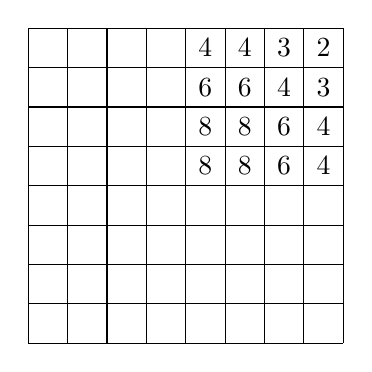
\begin{tikzpicture}[scale=0.5]
      \foreach \x in {0,1,...,8} {
        \draw (0, \x) -- (8, \x);
        \draw (\x, 0) -- (\x, 8);
      }
      \node at (7.5, 7.5) {$2$};
      \node at (7.5, 6.5) {$3$};
      \node at (6.5, 7.5) {$3$};
      \node at (6.5, 6.5) {$4$};

      \node at (7.5, 5.5) {$4$};
      \node at (7.5, 4.5) {$4$};
      \node at (5.5, 7.5) {$4$};
      \node at (4.5, 7.5) {$4$};

      \node at (6.5, 5.5) {$6$};
      \node at (6.5, 4.5) {$6$};
      \node at (4.5, 6.5) {$6$};
      \node at (5.5, 6.5) {$6$};

      \node at (4.5, 4.5) {$8$};
      \node at (4.5, 5.5) {$8$};
      \node at (5.5, 4.5) {$8$};
      \node at (5.5, 5.5) {$8$};
    \end{tikzpicture}
  \end{center}
  The sum of degrees is
  \[
    \sum_i d_i = 336.
  \]
  So the invariant distribution at, say, the corner is
  \[
    \pi_{\mathrm{corner}} = \frac{2}{336}.
  \]
\end{eg}
\end{document}
